
%%%%%%%%%%%%%%%%%%%%%%%%%%%%%%%%%%%%%%%%%%%%%%%%%%%%%%%%%%%%%%%%%%%%%%%%%%%%
% AGUJournalTemplate.tex: this template file is for articles formatted with LaTeX
%
% This file includes commands and instructions
% given in the order necessary to produce a final output that will
% satisfy AGU requirements, including customized APA reference formatting.
%
% You may copy this file and give it your
% article name, and enter your text.
%
%
% Step 1: Set the \documentclass
%
%

%% To submit your paper:
\documentclass[draft]{agujournal2019}
\usepackage[utf8]{inputenc}
\usepackage{url} %this package should fix any errors with URLs in refs.
\usepackage{lineno}
\usepackage[inline]{trackchanges} %for better track changes. finalnew option will compile document with changes incorporated.
\usepackage{soul}
\usepackage{amsmath}
\linenumbers

\definecolor{psign}{rgb}{0.9  ,0.1,0.1}
\definecolor{pregime}{rgb}{0.9,0.5,0.0}
\definecolor{pregimet}{rgb}{0.6,0.2,0.2}
\definecolor{pexpo}{rgb}{0.1,0.4,0.7}

\newcommand{\op}{\operatorname}

\newcommand*\patchAmsMathEnvironmentForLineno[1]{%
  \expandafter\let\csname old#1\expandafter\endcsname\csname #1\endcsname
  \expandafter\let\csname oldend#1\expandafter\endcsname\csname end#1\endcsname
  \renewenvironment{#1}%
     {\linenomath\csname old#1\endcsname}%
     {\csname oldend#1\endcsname\endlinenomath}}%
\newcommand*\patchBothAmsMathEnvironmentsForLineno[1]{%
  \patchAmsMathEnvironmentForLineno{#1}%
  \patchAmsMathEnvironmentForLineno{#1*}}%
\AtBeginDocument{%
\patchBothAmsMathEnvironmentsForLineno{equation}%
\patchBothAmsMathEnvironmentsForLineno{align}%
\patchBothAmsMathEnvironmentsForLineno{flalign}%
\patchBothAmsMathEnvironmentsForLineno{alignat}%
\patchBothAmsMathEnvironmentsForLineno{gather}%
\patchBothAmsMathEnvironmentsForLineno{multline}%
}

%%%%%%%
% As of 2018 we recommend use of the TrackChanges package to mark revisions.
% The trackchanges package adds five new LaTeX commands:
%
%  \note[editor]{The note}
%  \annote[editor]{Text to annotate}{The note}
%  \add[editor]{Text to add}
%  \remove[editor]{Text to remove}
%  \change[editor]{Text to remove}{Text to add}
%
% complete documentation is here: http://trackchanges.sourceforge.net/
%%%%%%%

% \draftfalse

%% Enter journal name below.
%% Choose from this list of Journals:
%
% JGR: Atmospheres
% JGR: Biogeosciences
% JGR: Earth Surface
% JGR: Oceans
% JGR: Planets
% JGR: Solid Earth
% JGR: Space Physics
% Global Biogeochemical Cycles
% Geophysical Research Letters
% Paleoceanography and Paleoclimatology
% Radio Science
% Reviews of Geophysics
% Tectonics
% Space Weather
% Water Resources Research
% Geochemistry, Geophysics, Geosystems
% Journal of Advances in Modeling Earth Systems (JAMES)
% Earth's Future
% Earth and Space Science
% Geohealth
%
% ie, \journalname{Water Resources Research}

\journalname{Journal of Advances in Modeling Earth Systems}


\begin{document}

%% ------------------------------------------------------------------------ %%
%  Title
%
% (A title should be specific, informative, and brief. Use
% abbreviations only if they are defined in the abstract. Titles that
% start with general keywords then specific terms are optimized in
% searches)
%
%% ------------------------------------------------------------------------ %%

% Example: \title{This is a test title}

\title{Weather and climate models in 16-bit arithmetics: Number formats, error mitigation and scope}

%% ------------------------------------------------------------------------ %%
%
%  AUTHORS AND AFFILIATIONS
%
%% ------------------------------------------------------------------------ %%

% Authors are individuals who have significantly contributed to the
% research and preparation of the article. Group authors are allowed, if
% each author in the group is separately identified in an appendix.)

% List authors by first name or initial followed by last name and
% separated by commas. Use \affil{} to number affiliations, and
% \thanks{} for author notes.
% Additional author notes should be indicated with \thanks{} (for
% example, for current addresses).

% Example: \authors{A. B. Author\affil{1}\thanks{Current address, Antartica}, B. C. Author\affil{2,3}, and D. E.
% Author\affil{3,4}\thanks{Also funded by Monsanto.}}

\authors{M. Kl\"{o}wer\affil{1}, P. D. D\"{u}ben\affil{2}, and T. N. Palmer\affil{1}}


% \affiliation{1}{First Affiliation}
% \affiliation{2}{Second Affiliation}
% \affiliation{3}{Third Affiliation}
% \affiliation{4}{Fourth Affiliation}

\affiliation{1}{Atmospheric, Oceanic and Planetary Physics, University of Oxford, Oxford, UK}
\affiliation{2}{European Centre for Medium-Range Weather Forecasts, Reading, UK}
%(repeat as many times as is necessary)

%% Corresponding Author:
% Corresponding author mailing address and e-mail address:

% (include name and email addresses of the corresponding author.  More
% than one corresponding author is allowed in this LaTeX file and for
% publication; but only one corresponding author is allowed in our
% editorial system.)

% Example: \correspondingauthor{First and Last Name}{email@address.edu}

\correspondingauthor{M. Kl\"{o}wer}{milan.kloewer@physics.ox.ac.uk}

%% Keypoints, final entry on title page.

%  List up to three key points (at least one is required)
%  Key Points summarize the main points and conclusions of the article
%  Each must be 140 characters or fewer with no special characters or punctuation and must be complete sentences

% Example:
% \begin{keypoints}
% \item	List up to three key points (at least one is required)
% \item	Key Points summarize the main points and conclusions of the article
% \item	Each must be 140 characters or fewer with no special characters or punctuation and must be complete sentences
% \end{keypoints}

\begin{keypoints}
\item $\circ$ Posit numbers have smaller rounding errors compared to floating-point numbers in weather and climate applications, enabling reliable shallow water simulations computed entirely with 16-bit arithmetic.

\item $\circ$ Errors caused by 16-bit floating-point arithmetic are strongly reduced with critical computations in 32 bit, which can be implemented on present-day hardware.

\item $\circ$ 16 or even 8-bit communication between processors, preferably encoded as posit numbers, introduces negligible errors, providing a perspective for reduced data communication for weather and climate models.

\end{keypoints}

%% ------------------------------------------------------------------------ %%
%
%  ABSTRACT and PLAIN LANGUAGE SUMMARY
%
% A good Abstract will begin with a short description of the problem
% being addressed, briefly describe the new data or analyses, then
% briefly states the main conclusion(s) and how they are supported and
% uncertainties.

% The Plain Language Summary should be written for a broad audience,
% including journalists and the science-interested public, that will not have
% a background in your field.
%
% A Plain Language Summary is required in GRL, JGR: Planets, JGR: Biogeosciences,
% JGR: Oceans, G-Cubed, Reviews of Geophysics, and JAMES.
% see http://sharingscience.agu.org/creating-plain-language-summary/)
%
%% ------------------------------------------------------------------------ %%

%% \begin{abstract} starts the second page

\begin{abstract}
The need for high precision calculations with 64-bit or 32-bit floating-point
arithmetic for weather and climate models is questioned.
Lower precision numbers can accelerate simulations and are increasingly supported
by modern computing hardware. This paper investigates the potential of 16-bit
arithmetic when applied within a shallow water model that serves as a medium
complexity weather or climate application. There are several 16-bit number
formats that can potentially be used (IEEE half precision, BFloat16, posits,
integer and fixed-point). It is evident that a simple change to 16-bit arithmetic
will not be possible for complex weather and climate applications as it will
degrade model results by intolerable rounding errors that cause a stalling of
model dynamics or model instabilities. However, if the posit number format is
used as an alternative to the standard floating-point numbers the model degradation
can be reduced to a tolerable minimum. Furthermore, a number of mitigation methods,
such as rescaling, reordering and mixed-precision, are available to make model
simulations resilient against a precision reduction. If mitigation methods are applied,
16-bit floating-point arithmetic can be used successfully within the shallow water model.
The results show the potential of 16-bit formats for at least parts of complex weather
and climate models where rounding errors would be entirely masked by intitial
condition, model or discretization error.

\end{abstract}

%% ------------------------------------------------------------------------ %%
%
%  TEXT
%
%% ------------------------------------------------------------------------ %%

\section*{Plain Language Summary}

64-bit floating-point numbers are the standard number format for scientific
computing in fluid dynamics, which allows for very precise calculations with
negligible rounding errors. The need for calculations at this precision level
has been questioned for weather and climate models, as errors are caused
primarily by insufficient observations or deficiencies of the models themselves.
Reducing numerical precision can accelerate simulations and low precision number
formats are increasingly supported by modern computers. This paper investigates
the potential of low numerical precision with numbers that only use 16 bit of
information, when applied within weather and climate applications. There are
several 16-bit number formats that can potentially be used, all of which have
considerably larger rounding errors than the standard 64-bit numbers. In this
paper, the different number formats are applied in a two-dimensional oceanic or
atmospheric circulation model. A simple change to 16-bits for all calculations
will not be possible as it will degrade simulation results. However, if mitigation
methods are applied, 16-bit calculations can be used successfully within the
applications of this paper. The results show the potential of 16-bit number
formats for at least parts of complex weather and climate models.

\section{Introduction}
\label{sec:intro}

Weather and climate models provide predictions that are of great importance for society and economy. The Earth's climate system remains very difficult to predict even with the computational resources of the world's largest supercomputers, due to its complexity and non-linear dynamics that couple all features from the smallest time and length-scales to the largest. The forecast error of a weather forecast model has several origins \cite{Palmer2012,Palmer2015}: (i) Initial and boundary condition errors, which result from observations, data assimilation, model errors and external factors; (ii) model error, i.e. the difference between the mathematical model and the real world; (iii) discretisation error resulting from a finite spatial and temporal resolution of the discretised equations and (iv) rounding errors with finite precision arithmetic. In general, the forecast error is dominated by (i-iii), depending on the forecast variable and the forecast lead time. In contrast, rounding errors are usually negligible if the IEEE 754 standard on 64 bit double precision floating-point numbers (Float64) is used, which is the standard for the majority of operational weather forecasts and in climate models.

Research on reduced precision floating-point arithmetics is motivated by the potential for faster processing and communication between different elements of the computing architecture. The gained speed can be traded for increased complexity of simulations, resulting in more accurate predictions of weather and climate. The Integrated Forecast System at the European Centre for Medium-Range Weather Forecasts can be run almost entirely with 32-bit single precision (Float32) without a decrease in forecast skill \cite{Vana2017}, but in 60\% of the run-time. Similar progress was made at MeteoSwiss with their weather forecast model COSMO \cite{Rudisuhli2013}. For the European ocean model NEMO a mix of 32-bit and 64-bit arithmetic is a promising approach to keep accuracy-critical parts in high precision while increasing performance in others \cite{TintoPrims2019}.

The recent boom of deep learning techniques, that require low numerical precision but high computational performance, is pushing hardware development to offer more flexibility for the use of reduced precision number formats. While 16-bit arithmetic was not available for use on commodity supercomputing hardware in the past, today most hardware vendors offer the use of 16-bit formats on the next generation of hardware. Graphic processing units started to support Float16 for increased performance \cite{Markidis2018}. Google's tensor processing units (TPU, \citeA{Jouppi2017,Jouppi2018}) support the 16-bit BFloat16 format, a truncated version of Float32, as this format is sufficient for many deep learning applications \cite{Kalamkar2019,Burgess2019,Gupta2015}.

Using simplistic chaotic models, it was shown that the majority of 64 bits with Float64 do not contain real information \cite{Jeffress2017}. Running algorithms used for weather forecast models at precision lower than 32 bit, for example with 16-bit half precision floats (Float16), is an active field of research, but remains challenging \cite{Duben2014,Thornes2017,Hatfield2018,Duben2018}. Most research on reduced precision modelling for weather and climate applications makes use of software emulators \cite{Dawson2017} that provide other arithmetics than Float32 and Float64 which are widely supported on today's hardware. This comes with the disadvantage that simulations are orders of magnitude slower. However, software emulation allows a scientific evaluation of the use of reduced numerical precision for weather and climate simulations with no need to port the models to special hardware (such as FPGAs, \citeA{Russell2017}).

Posit\texttrademark ~numbers are a recently proposed alternative to floating point numbers and claim to provide more precision in arithmetic calculations with fewer bits in algorithms of linear algebra or machine learning \cite{Gustafson2017,Langroudi2019}. However, posits remain untested for weather and climate simulations.

To get a better impression whether 16-bit arithmetic can be useful within weather and climate applications, which 16-bit formats are most promising, and how model simulations can be made resilient against a reduction in precision to 16 bits, this study will apply common types of 16-bit arithmetic in weather and climate applications and test approaches to mitigate negative impact if 16-bit arithmetic cannot be used for the entire model.

The paper is structured as follows: Section \ref{sec:formats} outlines the different number formats, the concept of decimal precision, and mitigation methods how weather and climate models can be made resilient against a reduction of numerical precision to 16-bit formats. Section \ref{sec:runs} presents results for the use of 16-bit arithmetic in a chaotic model at low complexity -- namely the Lorenz 1963 system -- and a model of medium complexity -- namely the shallow water equations. The mitigation methods are applied to the two models to reduce the impact of the precision reduction. Section \ref{sec:discuss} discusses the results and provides the conclusions.


\section{16-bit number formats and mitigation methods}
\label{sec:formats}

This section discusses different types of 16-bit arithmetic, and similarities
and differences between them. Mitigation methods that allow for the use of 
16-bit arithmetic within weather and climate applications are introduced.

\subsection{16-bit number formats}

\subsubsection{The integer and fixed point number format}
\label{sec:integer}

The simplest way to represent a real number in bits is the integer format.
An $n$-bit signed integer starts with a sign bit followed by a sequence of integer
bits, that are decoded as a sum of powers of 2 with exponents $0,1,...,n-2$.
The largest representable number $maxpos$ for a signed integer format is $2^{n-1}-1$.
Fixed-point numbers extend the integer format by adding $n_f$ fraction bits to
decode an additional sum of powers of 2 with negative exponents $-1,-2,...,-n_f$.
Every additional fraction bit reduces the number of integer bits. For example,
Q6.10 is the 16-bit fixed-point format with 6 signed integer bits and 10 fraction bits.

The arithmetic of fixed-point numbers is very similar to integers. The range of 
representable numbers with integer arithmetic can therefore be
changed with fixed-point numbers, providing some flexibility for integer arithmetics
\cite{Russell2017}. However, the width of the dynamic range $\log_{10}(maxpos/minpos)$
is always limited and less than five orders of magnitude for any 16-bit integer
or fixed-point format -- too small for most applications. We will therefore focus
on the discussion of the other number formats in the rest of the study.

\subsubsection{The floating-point number format}
\label{sec:floats}

The IEEE standard on floating-point arithmetic defines how floats encode a real
number $x$ in terms of a sign, and several exponent and significant bits
\begin{equation}
x = (-1)^{sign~bit} \cdot 2^{e-bias} \cdot (1+f).
\label{eq:float}
\end{equation}
The exponent bits $e$ are interpreted as unsigned integers, such that $e-bias$
converts them effectively to signed integers. The fraction (or significant) bits
$f_i$ are defined as before, such that the significand $(1+f)$ is in the bounds
$[1,2)$. An 8-bit float encodes a real number with a sign bit (red), $n_e = 3$
exponent bits (blue) and $n_f=4$ fraction bits (black) as illustrated in the
following example
\begin{equation}
3.14 \approx {\color{psign}0}{\color{pexpo}100}1001_{\op{Float8}} =
(-1)^{\color{psign}0} \cdot 2^{{\color{pexpo}4}-bias} \cdot (1+2^{-1}+2^{-4}) =
3.125
\label{eq:posit_pos}
\end{equation}
with $bias=2^{n_e-1} - 1 = 3$. Exceptions to Eq. \ref{eq:float} occur for
subnormal numbers, infinity (Inf) and Not-a-Number (NaN) when all exponent bits
are either zero (subnormals) or one (Inf when f=0, or NaN else). 16-bit half-precision
floating point numbers (Float16) have 5 exponent bits and 10 significant bits.
A truncated version of the Float32 format (8 exponent bits, 23 significant bits)
is BFloat16 with 8 exponent bits and 7 signficant bits. A format with more exponent
bits has a wider dynamic range of representable numbers but lower precision, as
fewer bits are available for the significand. All floating-point formats have a
fixed number of bits in the significand, consequently, they have a constant
number of significant digits throughout their range of representable numbers
(subnormals excluded).

\subsubsection{The posit number format}
\label{sec:posit_methods}

Posit numbers arise from a projection of the real axis onto a circle (Fig. \ref{fig:circle}),
with only one bitpattern for zero and one for complex infinity (or Not-a-Real, NaR),
which serves as a replacement for Not-a-Number (NaN). The circle is split into
\emph{regimes}, determined by a constant $useed$, which always marks the north-west
on the posit circle (Fig. \ref{fig:circle}b). Regimes are defined by
$useed^{\pm1}$, $useed^{\pm2}$, $useed^{\pm3}$, etc. which set a wide dynamic range of
representable numbers. To encode these regimes into bits, posit numbers use regime bits 
which extend the standard on floating-point arithmetic. Regime bits are a sequence of 
identical bits after the sign bit, terminated by an opposite bit. As the number 
of regime bits is not fixed but flexible, The significand increases in length for numbers
towards $\pm1$, when fewer regime bits are needed. Consequently, a higher precision around 
one can be achieved with posits, which is traded against a gradually lower precision for 
very large or very small numbers.

A positive posit number $p$ is decoded as \cite{Gustafson2017,Gustafson2017a,Chen2018,Klower2019}
\begin{equation}
p = (-1)^{sign~bit} \cdot useed^k \cdot 2^e \cdot (1+f).
\label{eq:posit}
\end{equation}
$k$ is the number of regime bits. $e$ is the unsigned integer represented by the exponent bits and $f$ is the fraction which is encoded in the fraction (or significant) bits. The number of exponent bits $e_s$ determines the base $useed = 2^{2^{e_s}}$ of the regime bits. More exponent bits increase - by increasing $useed$ - the dynamic range of representable numbers at the cost of precision. The exponent bits themselves fill gaps of powers of 2 spanned by $useed = 4,16,256,...$ for $e_s=1,2,3,...$ and so do not affect the dynamic range directly by changing the value of $2^e$ in Eq. \ref{eq:posit}. Consequently, every posit number, except for zero and NaR, can be written as $p = \pm 2^i \cdot (1+f)$ for a given integer $i$. In the following, a posit number format with $n$ bits including $e_s$ exponent bits is denoted as Posit($n$,$e_s$).

We provide an example in the Posit(8,1)-system (i.e. $useed = 4$), which encodes the number 14 as follows
\begin{equation}
{\color{psign}0}{\color{pregime}11}{\color{pregimet}0}{\color{pexpo}1}110_{\op{Posit}(8,1)} = (-1)^{\color{psign}0} \cdot 4^{\color{pregime}1} \cdot 2^{\color{pexpo}1} \cdot (1+2^{-1}+2^{-2}) = 14.
\label{eq:posit_pos}
\end{equation}
The sign bit is given in red, regime bits in orange, the terminating regime bit in brown, the exponent bit in blue and the fraction bits in black. The $k$-value is inferred from the number of regime bits, which are counted as negative for the bits being 0, and positive, but subtract 1, for the bits being 1. The exponent bits are interpreted as unsigned integer and the fraction bits follow the IEEE floating-point standard for significant bits.

\begin{figure}[htbp]
\center
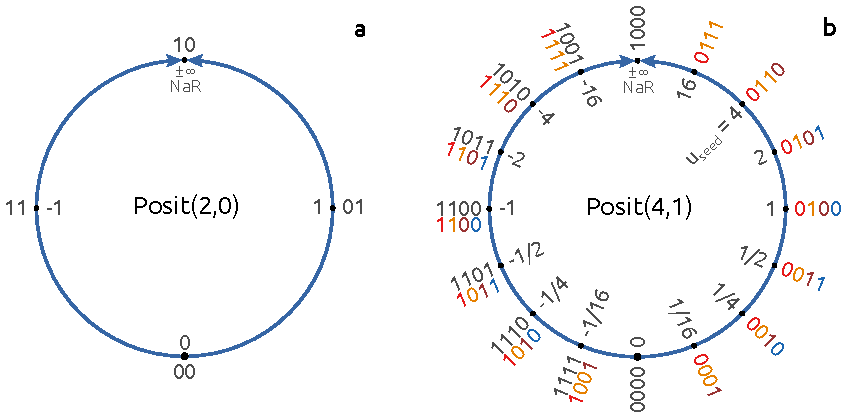
\includegraphics[width=1\textwidth]{circles.pdf}
\caption{Two posit number formats obtained by projecting the real axis onto a circle. (a) 2-bit Posit(2,0) and (b) 4-bit Posit(4,1). The bit patterns are marked on the outside and the respective values on the inside of each circle. Bit patterns of negative numbers (black) have to be converted to their two's complement (colours) first (see text). At the top of every circle is complex infinity ($\pm \infty$) or NaR (Not-a-Real). After \citeA{Gustafson2017a}.}
\label{fig:circle}
\end{figure}

In order to use posits on a conventional processor we developed for the Julia programming language \cite{Bezanson2017} the posit emulator \emph{SoftPosit.jl} \cite{Klower2019a}, which is a wrapper for the C-based library SoftPosit \cite{Leong2020}. A standardized posit processor is not yet available, but current research focuses on hardware implementations \cite{Zhang2020,vanDam2019,Chen2018,Chaurasiya2018,Glaser2017}.

\subsection{The concept of decimal precision and summary of number formats}
\label{sec:decprec}

Most arithmetic operations include rounding of an exact result $x_\text{exact}$
to a representable number $x_\text{repr}$. Based on the decimal rounding error
$\vert \log_{10}( \tfrac{x_\text{repr}}{x_\text{exact}} ) \vert$ the decimal precision
is defined as \cite{Gustafson2017}
\begin{equation}
\op{decimal} \op{precision} = -\log_{10} \vert \log_{10}( \frac{x_\text{repr}}{x_\text{exact}} ) \vert
\end{equation}
which measures the number of correct decimal places after rounding. The decimal precision tends to infinity when the representable number approaches the exact result. An exact result in between two representable numbers minimises the decimal precision as the decimal error is maximised. This minimum defines the \emph{worst-case} decimal precision, i.e. the number of decimal places that are at least correct after rounding. In the following we will refer to the worst-case decimal precision simply as decimal precision.
The machine epsilon $\epsilon$, a relative rounding error in floating-point arithmetic,
is commonly used to measure the precision of number formats. It is defined as the
distance $\delta$ between 1 and the next largest representable number, and can be
given in terms of decimal precision as $\epsilon = -\log_{10} ( \log_{10}( 1 + \tfrac{\delta}{2} ))$.

\begin{figure}[htbp]
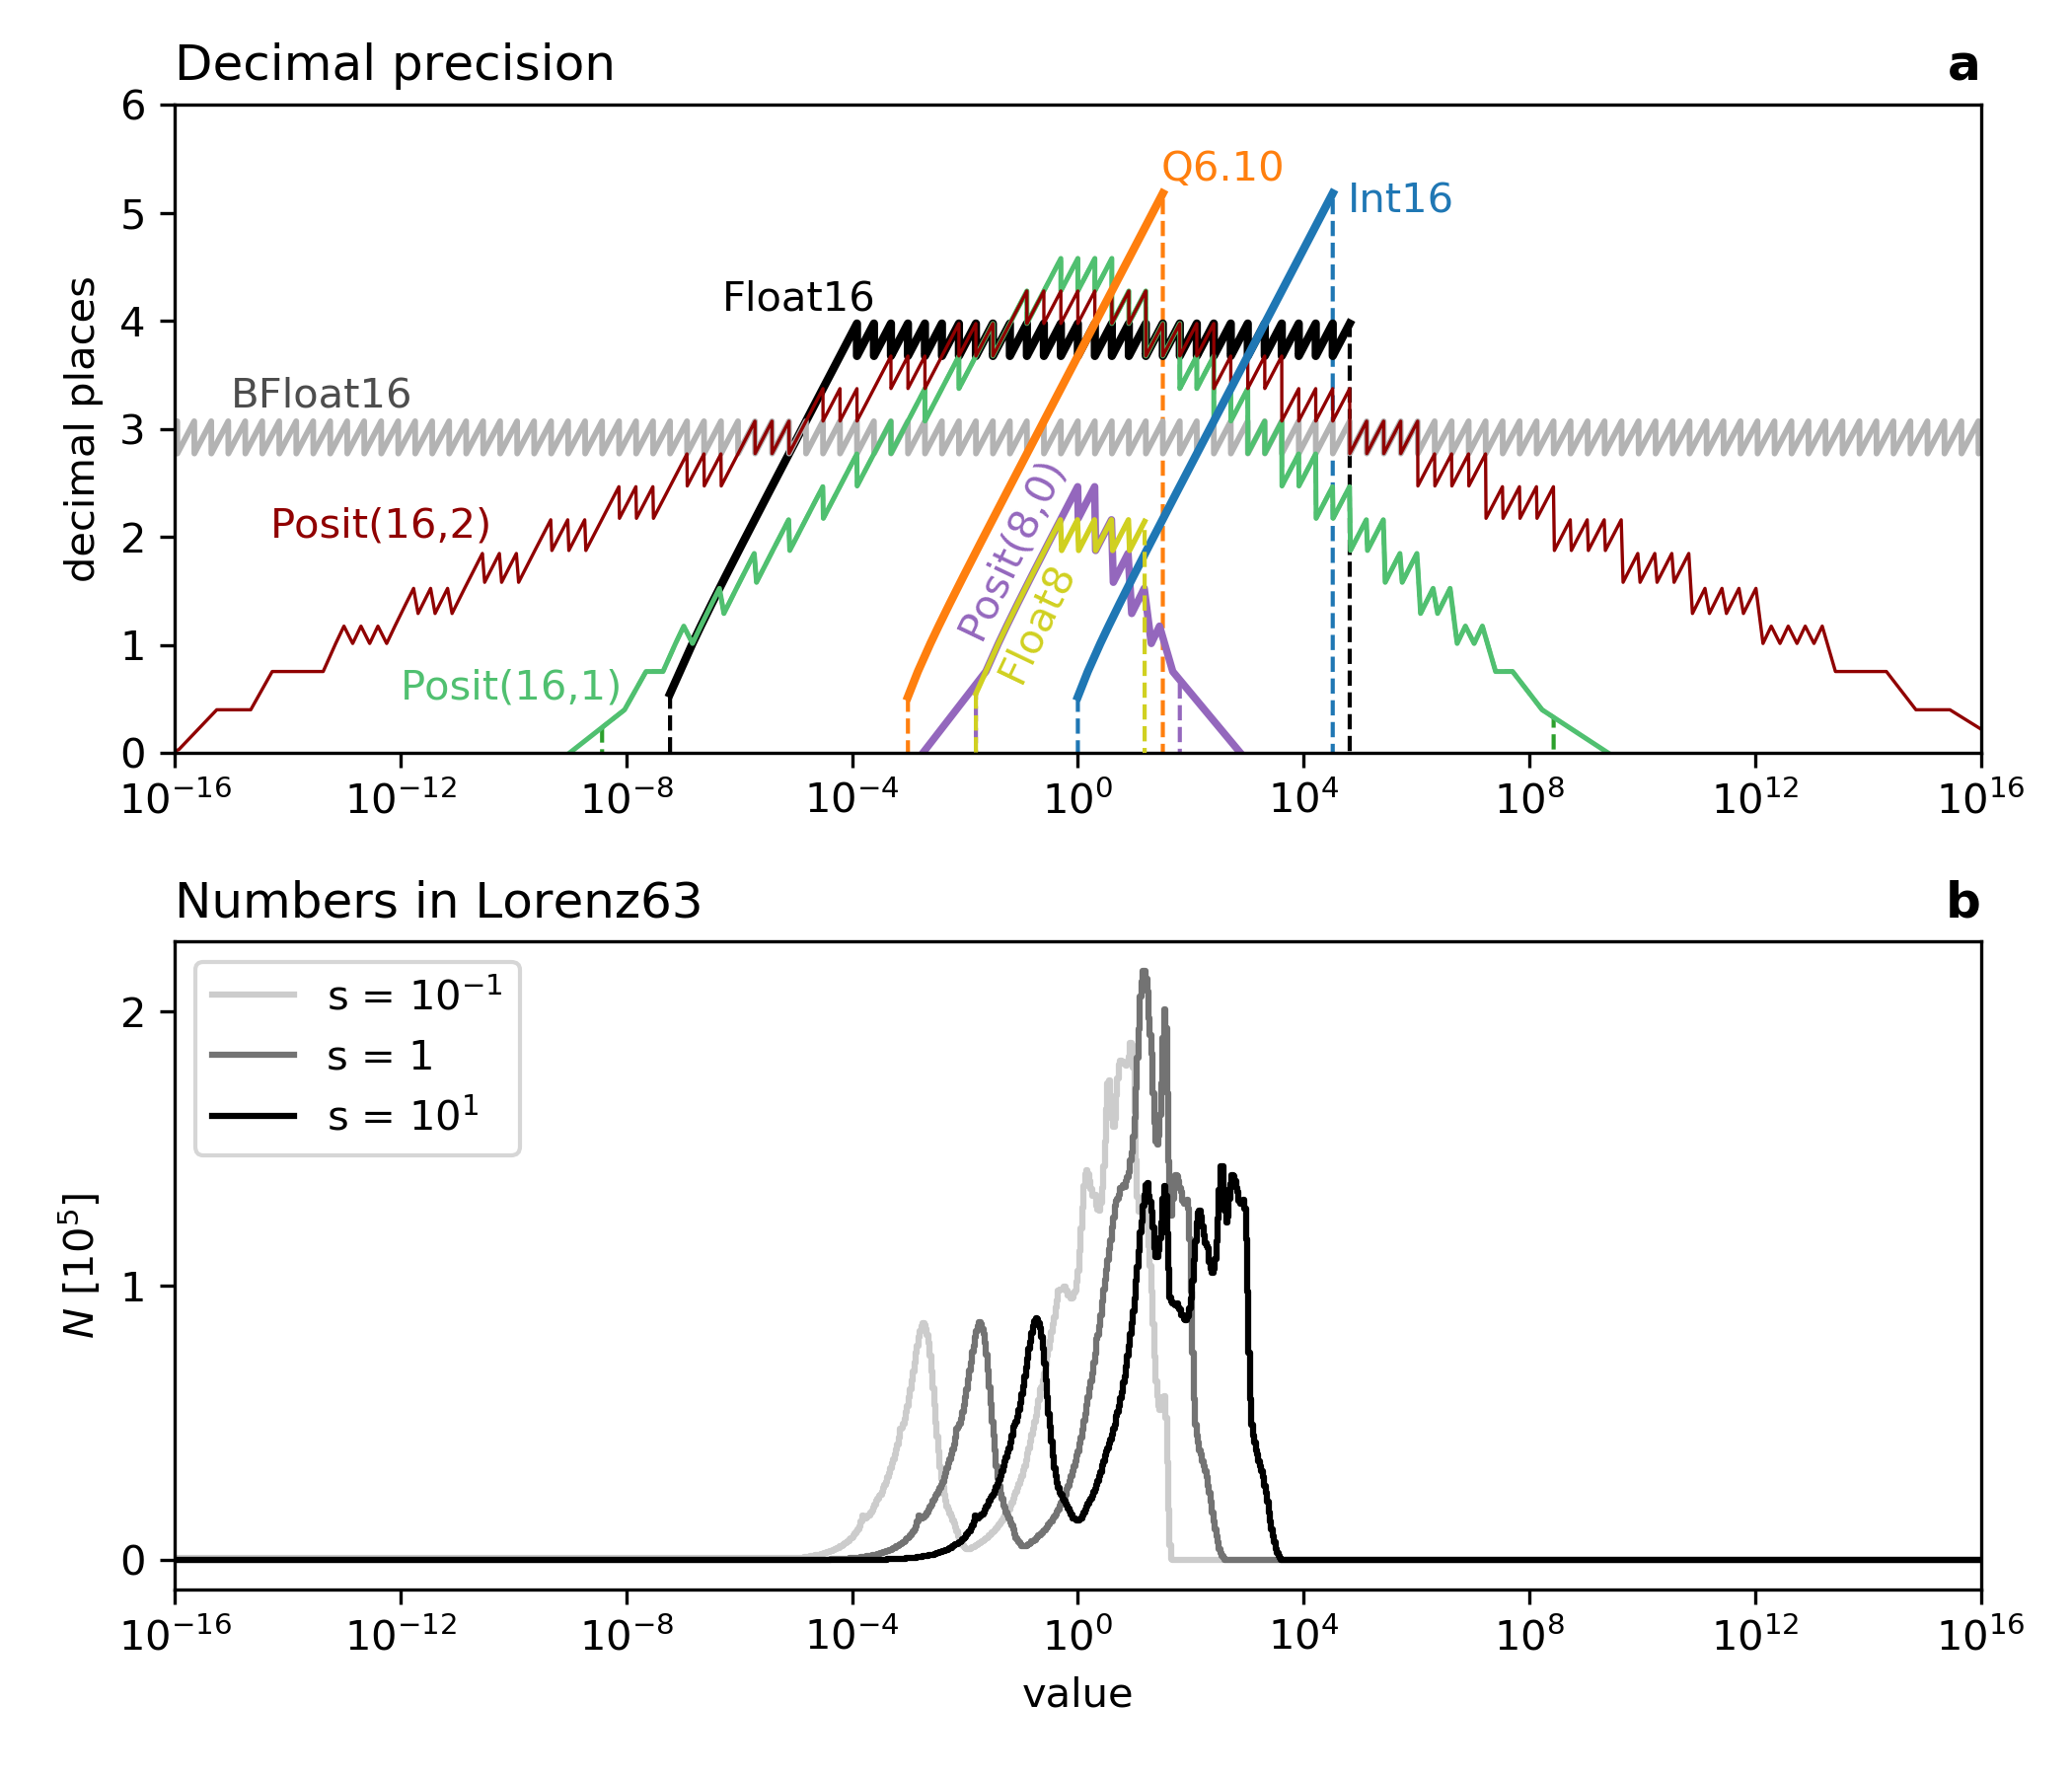
\includegraphics[width=1\textwidth]{decimal_precision.png}
\caption{(a) Decimal precision of various number formats. Dashed vertical lines indicate the range of representable numbers for each format. Float64, Float32 and Posit32 are beyond the axes limits. (b) Histogram of results of all arithmetic operations in the rescaled Lorenz system, considering absolute values.}
\label{fig:dec_prec}
\end{figure}

The decimal precision for various 16 and 8-bit floats and posits, 16-bit integers
and the fixed-point format Q6.10 (6 integer bits, 10 fraction bits) is presented
in Fig. \ref{fig:dec_prec}a. Floats have an exponent that is linearly-spaced in
log-space, which results in a nearly constant decimal precision. The deviations
from a constant decimal precision, which can be seen as spikes in Fig. \ref{fig:dec_prec}a,
are due to a linearly-spaced significant. The decimal precision for flats decreases
for the subnormal numbers towards the smallest representable number $minpos$.
Posits have an increased decimal precision around 1 and a yet a wide dynamic range,
due to the tapered precision towards $minpos$ and the largest representable number
$maxpos$. The decimal precision for posits is above zero outside the dynamic range as posits
have a no overflow/no underflow-rounding mode. Integers are linearly-spaced,
consequently their precision increases towards $maxpos$,
which is $2^{15} - 1 =  32767$ for 16-bit signed integers. The decimal precision of
fixed-point numbers has an identical shape, but shifted towards smaller numbers
by a factor of $\tfrac{1}{2}$ for each additional fraction bit. Consequently,
many arithmetic calculations should be placed close to $maxpos$, but the small
range of high precision is restrictive for many applications. No convincing results
with integer or fixed-point arithmetic was achieved in this study.

\begin{table}[htbp]
\center
\begin{tabular}{l | r | r | l | l | r | r}
Format & bits & exp bits & $minpos$ & $maxpos$ & $\epsilon$ &  \% NaR \\
\hline
Float64	& 64 & 11 & $5.0 \cdot 10^{-324}$ & $1.8 \cdot 10^{308}$  & 16.3 & 0.0 \\
Float32	& 32 & 8 & $1.0 \cdot 10^{-45}$ & $3.4 \cdot 10^{38}$ & 7.6 & 0.4 \\
Float16	& 16 & 5 & $6.0 \cdot 10^{-8}$ & 65504 & 3.7 & 3.1 \\
BFloat16	& 16 & 8 & $ 9.2 \cdot 10^{-41}$ & $3.4 \cdot 10^{38}$ & 2.8 & 0.4  \\
Float8 & 8 & 3 & $1.5 \cdot 10^{-2}$ & 15.5 & 1.9 &12.5\\
\hline
Posit32	& 32 & 2 &  $7.5 \cdot 10^{-37}$ & $7.5 \cdot 10^{37}$ & 8.8 & 0.0 \\
Posit(16,1) & 16 & 1 & $3.7 \cdot 10^{-9}$ & $3.7 \cdot 10^{9}$ & 4.3 & 0.0\\
Posit(16,2) & 16 & 2 & $1.4 \cdot 10^{-17}$ & $1.4 \cdot 10^{17}$ & 4.0 & 0.0\\
Posit(8,0) & 8 & 0 & $1.5 \cdot 10^{-2}$ & 64 & 2.2 & 0.4  \\
\hline
Int16 & 16 & 0 & 1 & 32767 & 0.8 & 0\\
Q6.10 & 16 & 0 & $9.8 \cdot 10^{-4}$ & 32.0 & 3.7 & 0
\end{tabular}
\vspace{10pt}
\caption{Some characteristics of various number formats. $minpos$ is the smallest representable positive number, $maxpos$ the largest. The machine error $\epsilon$ is here given as decimal precision. \% NaR denotes the percentage of bit patterns that represent not a number (NaN), infinity or not a real (NaR).}
\label{tab:formats}
\end{table}

Characteristics of various formats are summarised in Table \ref{tab:formats}. The machine error $\epsilon$, defined as half the distance between 1 and the next representable number, can be given in terms of decimal precision and is summarized in Table \ref{tab:formats} for the various formats. Float64 has more than $10^{15}$ bitpatterns reserved for NaN, but these only make up $< 0.05\%$ of all available bit patterns. However, the percentage of redundant bitpatterns for NaN increases for floats with fewer exponent bits and poses a noticable issue for Float16 and Float8.


\subsection{Mitigation measures to allow for the use of 16-bit arithmetic in weather and climate applications}

\subsubsection{Mixed precision arithmetic}

In many models, it will not be possible (or useful) to use 16-bit arithmetic
throughout the entire model. Some model components will be more sensitive to a
reduction in precision when compared to others and it often makes sense to reduce
precision only in those components where results are not deteriorated, while
keeping precision high in precision-sensitive components. This approach is
called \emph{mixed-precision} and is already used for the reduction to single
precision in ocean and atmosphere models \cite{Vana2017,TintoPrims2019}.

\subsubsection{Algorithmic changes: Rescaling, reordering and precomputations}

Equations can be \emph{rescaled} via multiplication with a constant rescaling
factor $s$ to shift the dynamic range occurring in an algorithm towards larger
numbers (for $s > 1$) or towards smaller numbers ($s < 1$). Rescaling can be used
to adjust the number range to the decimal precision of the number formats. If
non-linear terms are considered, this multiplicative rescaling is ineffective,
as the rescaling factor $s$ appears (as an additional multiplication with $s^{-1}$)
inside the non-linear terms. The non-linear terms are therefore effectively invariant
under multiplicate rescaling and only the linear terms are scaled by $s$.
Fig. \ref{fig:dec_prec} includes histograms of numbers occurring in the rescaled
Lorenz system \cite{Lorenz1963,Kwasniok2014,Jeffress2017,Tantet2018} as an example
from \citeA{Klower2019}. For posit arithmetic it is preferable to use
$s=\tfrac{1}{10}$ in the Lorenz system to scale the prognostic variables
to match the range of highest decimal precision around 1, which increases the
complexity of the Lorennz attractor and decreases the average rounding error.

Furthermore, it is sometimes possible to avoid intermediate arithmetic results,
which may be outside the dynamic range of a number format, by changing the order
in which multiplications and divisions are executed. In general, it is preferable
to combine such operations to a single multiplication with a constant, that can
be precomputed. Although this will have a negligible effect on the rounding error
for floating-point arithmetic due to the approximately constant decimal precision
throughout the range of numbers (subnormals excluded), it reduces the risk of
over- or underflow.

\subsubsection{Reduced precision communication}

Complex weather and climate models rely on parallelisation to distribute the
computational cost of simulations efficiently among the processing units in a
large cluster or supercomputer. Parallel execution typically requires domain
decomposition, where the spatial domain is split into many subdomains to be
calculated separately on individual processing units. Domain decomposition
requires communication of the boundary values of a subdomain with the
neighbouring subdomains. If 16-bit arithmetic cannot be used within the
entire model, it may still be possible to reduce precision in the communication
between processors.

Not all weather and climate models would benefit from a reduced precision
communication as the acceleration potential depends on many factors specific
to a model and the used hardware, e.g. number of nodes in a cluster and how
shared and distributed memory management is realized. It will also be important
whether communication is latency or volume bound. Latency bound communication is
bound by the time a package of information requires to travel between processors.
In contrast, volume bound communication is limited by the bandwidth that is
available for communication. Only the latter will benefit from a reduction in
precision and therefore data volume.

However, in the case that the volume of the communication is an identified
bottleneck in a given application, which is often the case in weather and
climate models, it is possible that reliable model simulations can be achieved
with 16 or even 8-bit communication allowing for a signficant reduction in
computing time. The range of values that are communicated can be adjusted,
facilitating a strong compression of the data that is communicated and
opening the door to communication in very low precision.

\section{A shallow water model with 16-bit arithmetic}
\label{sec:swm}

This section will evaluate the different number formats Float16, BFloat16, Posit(16,1) and Posit(16,2) when solving the shallow water equations. The shallow water equations result from a vertical integration of the Navier-Stokes equations under the assumption that horizontal length scales are much greater than vertical scales. This assumption holds for many features of the general circulation of atmosphere and ocean \cite{Gill1982,Vallis2006}. The shallow water equations for the prognostic variables velocity $\mathbf{u} = (u,v)$ and sea surface elevation $\eta$ are
\begin{subequations}
\begin{align}
\frac{\partial \mathbf{u}}{\partial t} &+ (\mathbf{u} \cdot \nabla) \mathbf{u} + f\hat{\mathbf{z}} \times \mathbf{u} = -g\nabla \eta + \mathbf{D} + \mathbf{F} \\
\frac{\partial \eta}{\partial t} &+ \nabla \cdot (\mathbf{u}h) = 0.
\end{align}
\label{eq:swe}%
\end{subequations}
For the atmosphere, $\eta$ is interpreted as pressure \cite{Gill1982}. The shallow water system is forced with a zonal wind stress $\mathbf{F}$. The dissipation term $\mathbf{D}$ removes energy on large scales (bottom friction) and on small scales (diffusion). The non-linear term $(\mathbf{u} \cdot \nabla) \mathbf{u}$ represents advection of momentum. The term $f\hat{\mathbf{z}} \times \mathbf{u}$ is the Coriolis force and $-g\nabla \eta$ is the pressure gradient force, with $g$ being the gravitational acceleration. Eq. \ref{eq:swe}b is the shallow water-variant of the continuity equation, ensuring conservation of mass.

The shallow water equations are solved in the $(x,y)$-plane over the zonally periodic rectangular domain $L_x \times L_y$, of size $2000\op{km} \times 1000\op{km}$. We associate $x$ with the zonal and $y$ with the meridional direction. The domain is centred at 45N and the beta-plane approximation \cite{Vallis2006} is used to linearize the Coriolis parameter which varies linearly from $9.5 \times 10^{-5}\op{s}^{-1}$ at the southern boundary to $1.1 \times 10^{-4}\op{s}^{-1}$ at the northern boundary. The boundary conditions are periodic in zonal direction and no-slip at the northern and southern boundary. The layer thickness is $h = \eta + H(x)$, with
\begin{equation}
H(x) = H_0 - H_1\exp\left(-H_\sigma^{-2}(x-\tfrac{L_x}{2})^2\right)
\end{equation}
being the undisturbed depth, representing a meridional mountain ridge at $x=\tfrac{L_x}{2}$ spanning from the southern to the northern boundary. The standard depth is $H_0 = 500\op{m}$. The ridge has a height of $H_1 = 50\op{m}$. The characteristic width of the ridge is $H_\sigma = 300\op{km}$. The time step $\Delta t = 282\op{s}$ is chosen to resolve surface gravity waves, traveling at an estimated phase speed of $\sqrt{gH_0}$ with CFL number being close to 1 and gravitational acceleration $g=10\op{ms}^{-1}$. The wind stress forcing $\mathbf{F} = (F_x,0)$ is constant in time, acts only on the zonal momentum budget
\begin{equation}
Fx = \frac{F_0}{\rho h} \cos\left(\pi\left(y{L_y}^{-1} - 1\right)\right)^2
\end{equation}
and vanishes at the boundaries. The water density is $\rho = 1000\op{kg}\op{m}^{-3}$ and $F_0 = 0.12\op{Pa}$. The dissipation term $\mathbf{D}$ is the sum
\begin{equation}
\mathbf{D} = -\frac{c_D}{h}\| \mathbf{u} \| \mathbf{u} - \nu \nabla^4 \mathbf{u}
\label{eq:diss}
\end{equation}
of a quadratic bottom drag with dimensionless coefficient $c_D = 10^{-5}$ \cite{Arbic2008} and a biharmonic diffusion with viscosity coefficient $\nu \approx 1.33\times10^{11} \op{m}^4\op{s}^{-1}$ \cite{Griffies2000}.

The shallow water equations are discretised using 2nd order centred finite differences on an Arakawa C-grid \cite{Arakawa1977} and the fourth order Runge-Kutta method \cite{Butcher2016} is used for time integration of the pressure, coriolis and advective terms, whereas a semi-implicit method is used for the dissipative terms $\mathbf{D}$. We present results of simulations with three different levels of resolution: high resolution simulations with a grid spacing of $\Delta = 5\operatorname{km}$ (400x200 grid points), medium resolution simulations with a grid-spacing of $\Delta = 20\operatorname{km}$ (100x50 grid points) and low resolution with a grid-spacing of $\Delta = 40\operatorname{km}$ (50x25 grid points). The advection terms are discretised using an energy and enstrophy conserving scheme \cite{Arakawa1990}.

To test the use of the different number formats for the representation of passive tracers in atmosphere and ocean, we extend the shallow water equations with an advection equation. Tracers could, for example, be temperature and salinity in the ocean or aerosols in the atmosphere, which are regarded here, for simplicity, as passive (i.e. they do not influence the flow). The change of the distribution of a passive tracer $q$ that is advected by the underlying flow field is described by
\begin{equation}
\frac{\partial q}{\partial t} + \mathbf{u} \cdot \nabla q = 0.
\label{eq:adv}
\end{equation}
We discretise Eq. \ref{eq:adv} with a semi-Lagrangian advection scheme \cite{Smolarkiewicz1992}, which calculates the tracer concentration for a given grid cell from the concentration at the previous time step at a departure point, which in turn is determined from the flow field. As the departure point is usually in between grid nodes an interpolation is required to find the concentration at the departure point, which is then the concentration at the arrival point.

\subsubsection{Rescaling the shallow water equations}
\label{sec:swm_rescale}

For 16-bit arithmetic it is essential to re-order the calculations in the shallow water equations to avoid calculations with very large or very small results, as the dynamic range of representable numbers is limited (Fig. \ref{fig:dec_prec}a and Table \ref{tab:formats}). This is especially true for some sophisticated schemes like the biharmonic diffusion \cite{Griffies2000}, which is often used to remove energy from the grid scale to ensure numerical stability. For biharmonic diffusion a fourth derivative in space is calculated. Due to the large dimension of geophysical applications, this term can get very small $\mathcal{O}(10^{-20})$ while viscosity coefficients are typically very large $\mathcal{O}(10^{11})$. The prognostic variables of Eq. \ref{eq:swe} and \ref{eq:adv} are typically $\mathcal{O}(1\op{ms}^{-1})$ for $\mathbf{u}$, $\mathcal{O}(1\op{m})$ for $\eta$ and $\mathcal{O}(1)$ for $q$. We therefore retain their physical units in the discretised numerical model and do not apply a rescaling of the shallow water equations. However, due to the grid spacing $\Delta$ of unit meter being large for geophysical flows, we need to use dimensionless Nabla operators $\tilde{\nabla} = \Delta\nabla$. The continuity equation Eq. \ref{eq:swe}b, for example, is discretised with an explicit time integration method as
\begin{equation}
\eta^{n+1} = \eta^n + RK_{\eta}\left( - \tilde{\nabla} \cdot (\mathbf{u}h)^n\right)
\label{eq:discr}
\end{equation}
where $RK_\eta$ is the Runge-Kutta coefficient times $\tfrac{\Delta t}{\Delta}$ which is precomputed at high precision, to avoid a division by a large value for $\Delta$ and a subsequent multiplication with a large value for $\Delta t$. The other terms are rescaled accordingly ($\tilde{f} = f\Delta$; $\tilde{\mathbf{F}} = \mathbf{F}\Delta$). As these terms remain constant, they are precomputed at higher precision during model initialisation to avoid problems with the dynamic range. To avoid division and subsequent multiplication with large numbers in the dissipative terms (Eq. \ref{eq:diss}) throughout the numerical model integration, we rescale $\mathbf{D}$  accordingly
\begin{equation}
\tilde{\mathbf{D}} =-\frac{\tilde{c_D}}{h}\| \mathbf{u} \| \mathbf{u} - \tilde{\nu}\tilde{\nabla}^4\mathbf{u}
\end{equation}
with $\tilde{c_D} = c_D\Delta = 0.2\op{m}$,  and $\tilde{\nu} = \nu\Delta^{-3} \approx 0.16\op{ms}^{-1}$, which are precomputed. Computing the term $\tilde{\mathbf{D}}$ instead of $\mathbf{D}$ is required to avoid arithmetic under and overflow with floats or huge rounding errors with posit arithmetic.

How to reformulate the semi-Lagrangian advection scheme for 16-bit arithmetics is explained in the following. This semi-Lagrangian advection scheme is based on the idea to solve the advection equation with respect to its Lagrangian formulation. In the absence of sources and sinks, the Lagrangian point-of-view states that the tracer concentration $q$ does not change following a flow trajectory. The concentration $q$ at departure points $\mathbf{x}_d$ at time $t$ is therefore the same as the concentration at time $t+\Delta t_{\op{adv}}$ at arrival points $\mathbf{x}_a$, which are chosen to coincide with the grid points. Based on the flow velocity at the arrival point, the departure point is derived. In order to avoid large numbers of the coordinates ($L_x = 2 \cdot 10^6$m), non-dimensional departure points $\mathbf{\tilde{x}}_{d,rel}$ relative to the arrival point are computed as
\begin{equation}
\mathbf{\tilde{x}}_{d,rel} = - \mathbf{u}(\mathbf{x}_a,t+\Delta t_{\op{adv}}) \left( \frac{\Delta t_{\op{adv}}}{\Delta} \right).
\label{eq:relcoord}
\end{equation}
A scaling with the grid-spacing inverse $\Delta^{-1}$ is applied such that all terms are $\mathcal{O}(1)$ and therefore representable with 16-bit arithmetics. In practice, when converting the relative departure point $\mathbf{\tilde{x}}_{d,rel}$ to an array index for the interpolation, the floor function is used in combination with integer arithmetics. This essentially separates a computation with reals into two parts. One that can be computed with integers without rounding errors, and a calculation with reals, with a removed offset to reduce rounding errors.

\subsubsection{Shallow water simulations in 16-bit arithmetic}

\begin{figure}
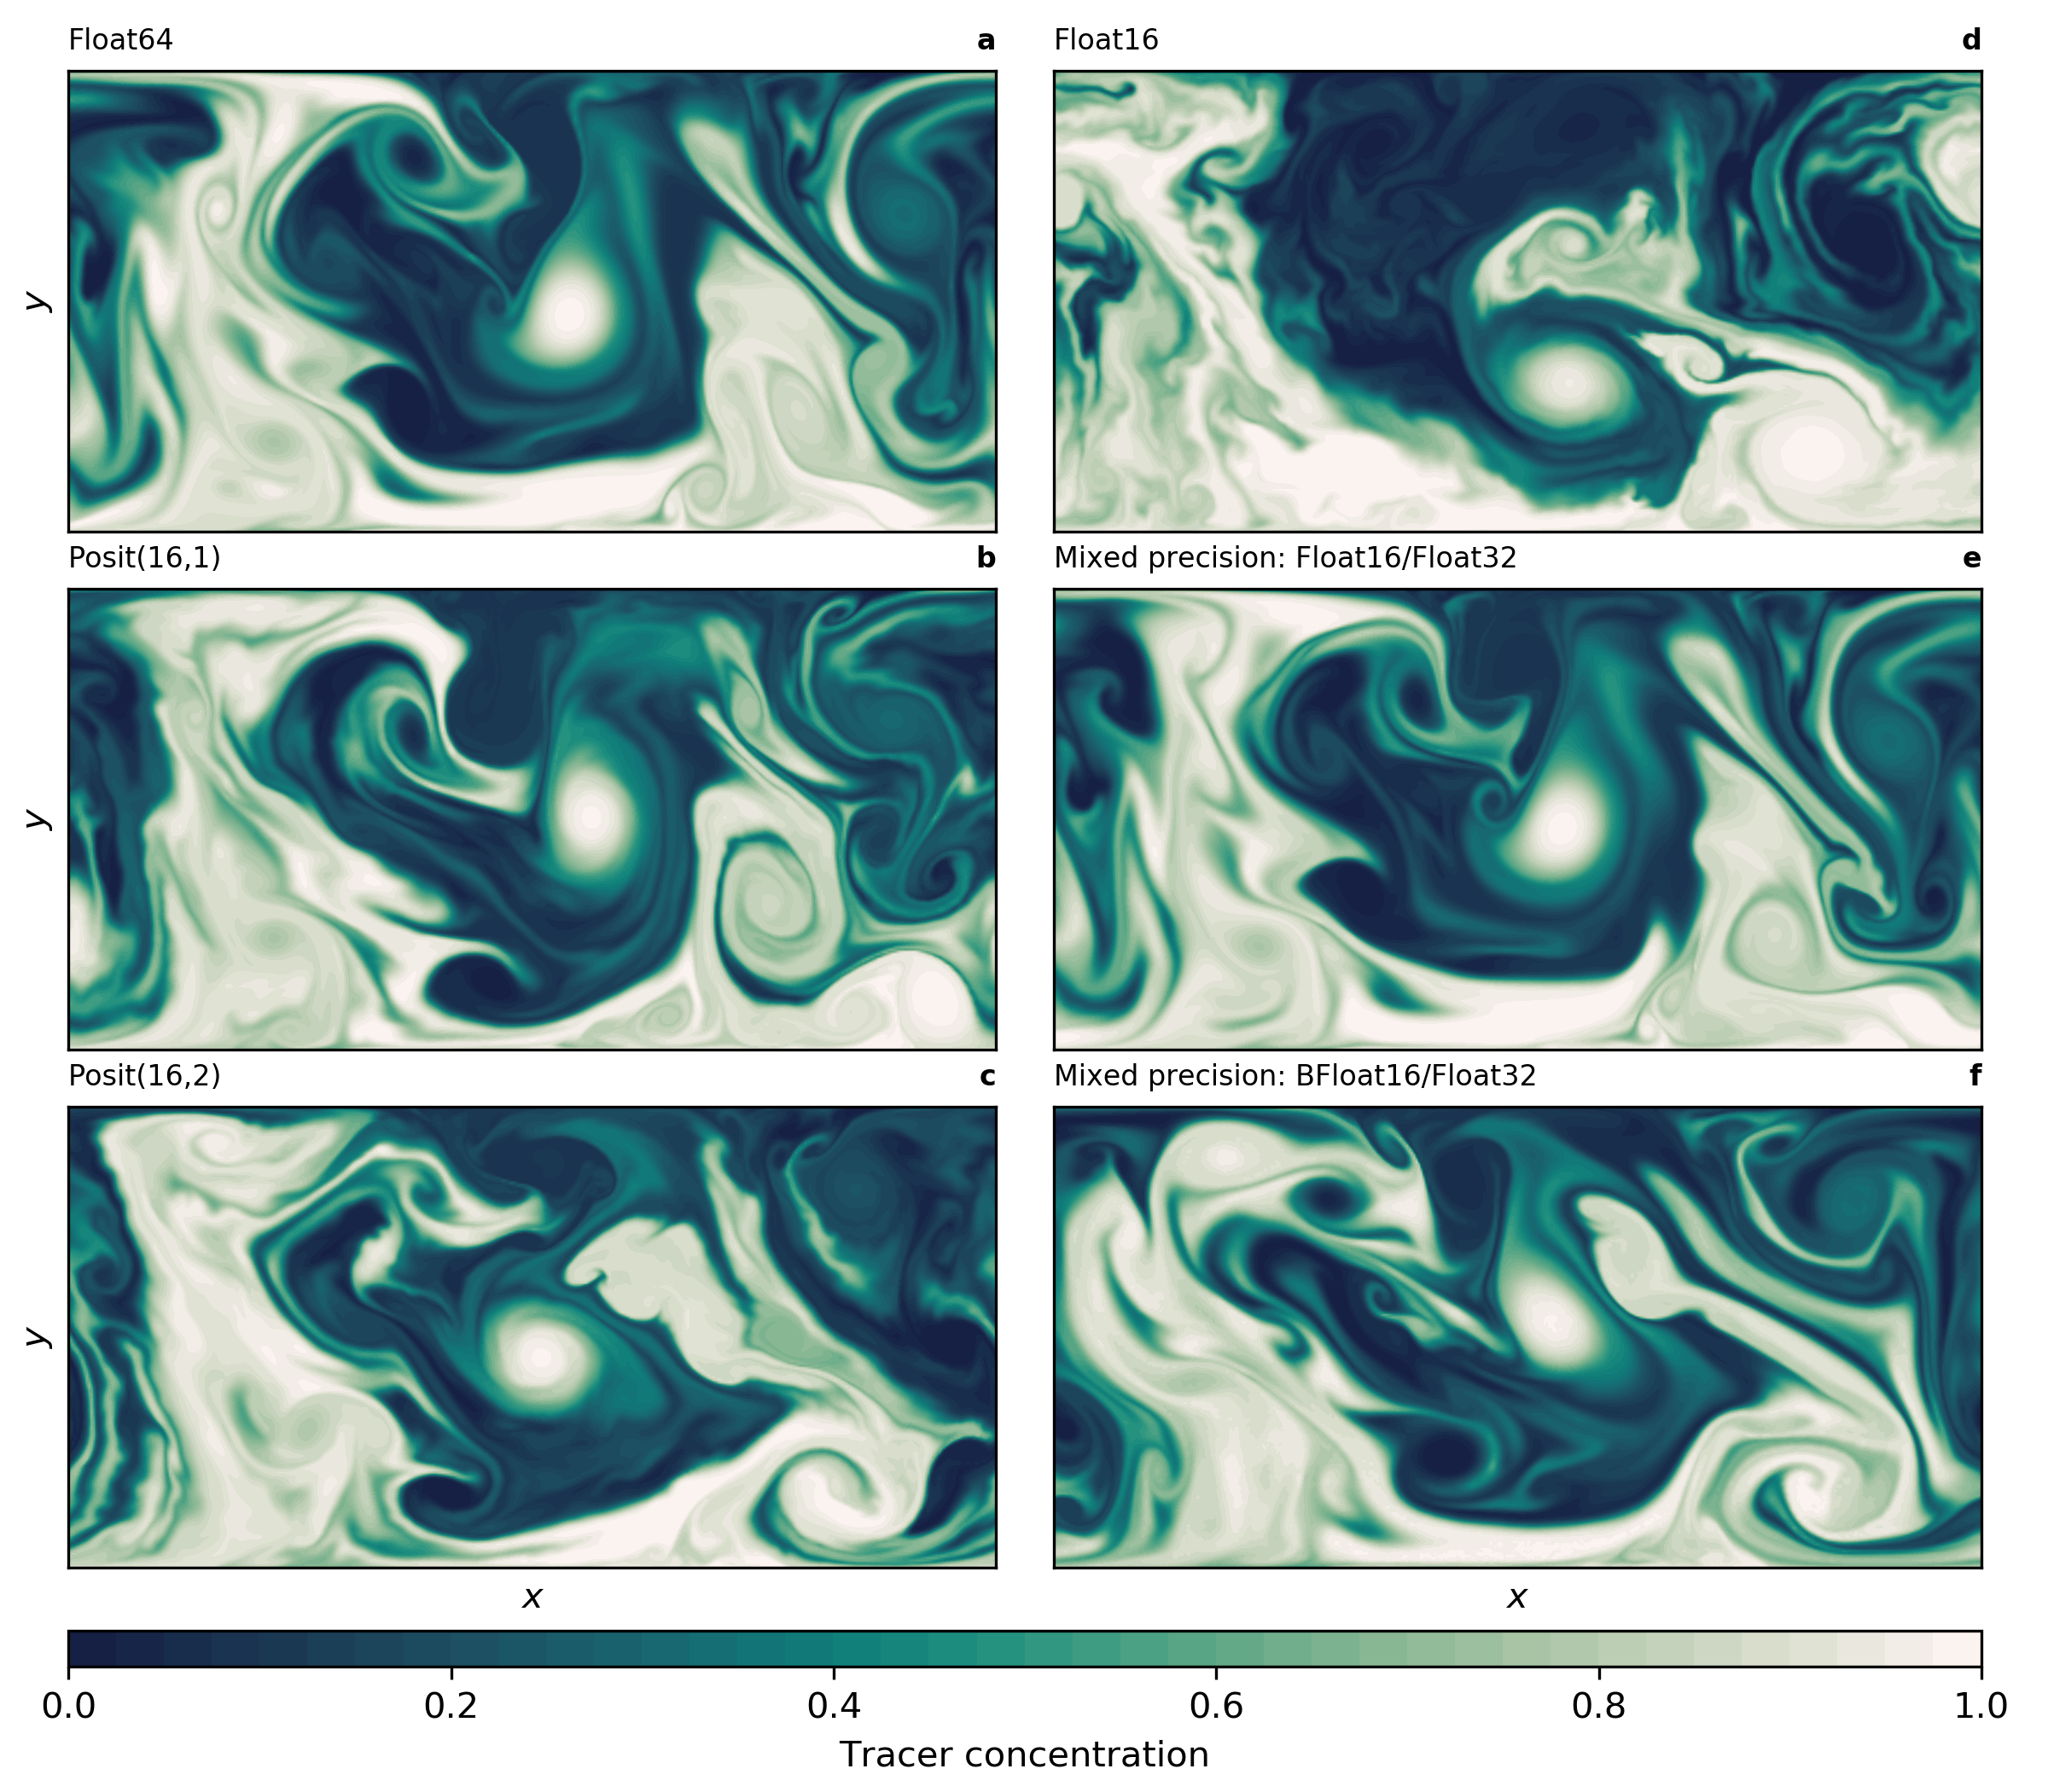
\includegraphics[width=1\textwidth]{snapshot.png}
\caption{Snapshot of tracer concentration simulated by the shallow water model using different 16-bit number formats and the medium-resolution configuration. The mixed precision simulations presented in (e) and (f) are using Float32 for the representation of prognostic variables only. The tracer was injected uniformly in the lower half of the domain 50 simulation days before the plot. These simulations were run in the high-resolution configuration.}
\label{fig:snapshot}
\end{figure}

The solution to the shallow water equations includes vigorous turbulence that dominates a meandering zonal current. Using either float or posit arithmetic in 16 bit the simulated fluid dynamics are very similar to a Float64 reference: As shown in a snapshot of tracer concentration (Fig. \ref{fig:snapshot}) turbulent stirring and mixing can be well simulated with posits. However, the Float16 simulation (Fig. \ref{fig:snapshot}d) deviates much faster than the posit simulations (Fig. \ref{fig:snapshot}b and c) from the Float64 reference (Fig. \ref{fig:snapshot}a), presumably due to the small scale instabilities visible in the snapshot as wavy filaments and fronts. These instabilities are clearly triggered by Float16 arithmetics, but to a lower degree also visible for posits. This provides a first evidence that the accumulated rounding errors with posits are smaller than with floats. BFloat16 arithmetic is not able to simulate the shallow water dynamics, presumably as tendencies are too small to be added to the prognostic variables, an issue that also occurs in the Lorenz system (Fig. \ref{fig:L63}d).

\begin{figure}
\includegraphics[width=1\textwidth]{rmse_eta_darker.pdf}
\caption{Forecast error measured as the root mean square error (RMSE) of sea surface height $\eta$ taking Float64 as reference. (a) Forecast error for various 16-bit number formats and mixed 16/32 bit simulations for which the prognostic variables are kept at Float32. (b) Forecast error for reduced precision communication in 8 or 16 bit with various number formats used for encoding, with Float64 used for all calculations.  The communication of boundary values occurs at every time step for the prognostic variables. The RMSE is normalised by a mean forecast error at very long lead times. Solid lines represent the median of 200 forecasts per number format. The shaded areas of each model configuration denote the interquartile range of the forecast experiments.}
\label{fig:rmse}
\end{figure}

To quantify differences between the different 16-bit arithmetics we perform short-term forecasts with the medium-resolution configuration. To quantify the error growth of rounding errors with different arithmetics in a statistically robust way, we create a number of forecasts with each member starting from one of 200 randomly picked start dates from a 50 year long control simulation. The forecast error in the shallow water model is computed as root mean square error (RMSE) of sea surface height with respect to Float64 simulations. Other variables yield similar results. Each forecast is performed several times from identical initial conditions but with the various number formats. To compare the magnitude of rounding error that are caused by a reduction in precision to a realistic level of error that is caused by model discretisation, we also perform forecasts with Float64 and the low-resolution model configuration, which are used to estimate the discretization error. We normalise the RMSE by the climatological mean forecast error at very long lead times, which is the same for all model configurations. A normalised RMSE of 1 therefore means that all information of the initial conditions is removed by chaos.

The forecast error of Float16 is as large as the discretisation error and clearly outperformed by 16-bit posit arithmetic (Fig. \ref{fig:rmse}a). Both Posit(16,1) and Posit(16,2) yield a forecast error that is several times smaller than Float16. The forecast error of 32-bit arithmetic is several orders of magnitude smaller and is only after 200 days as large as the error for 16-bit arithmetic at very short lead times. Also at 32 bit, posits clearly outperform floats.

\begin{figure}
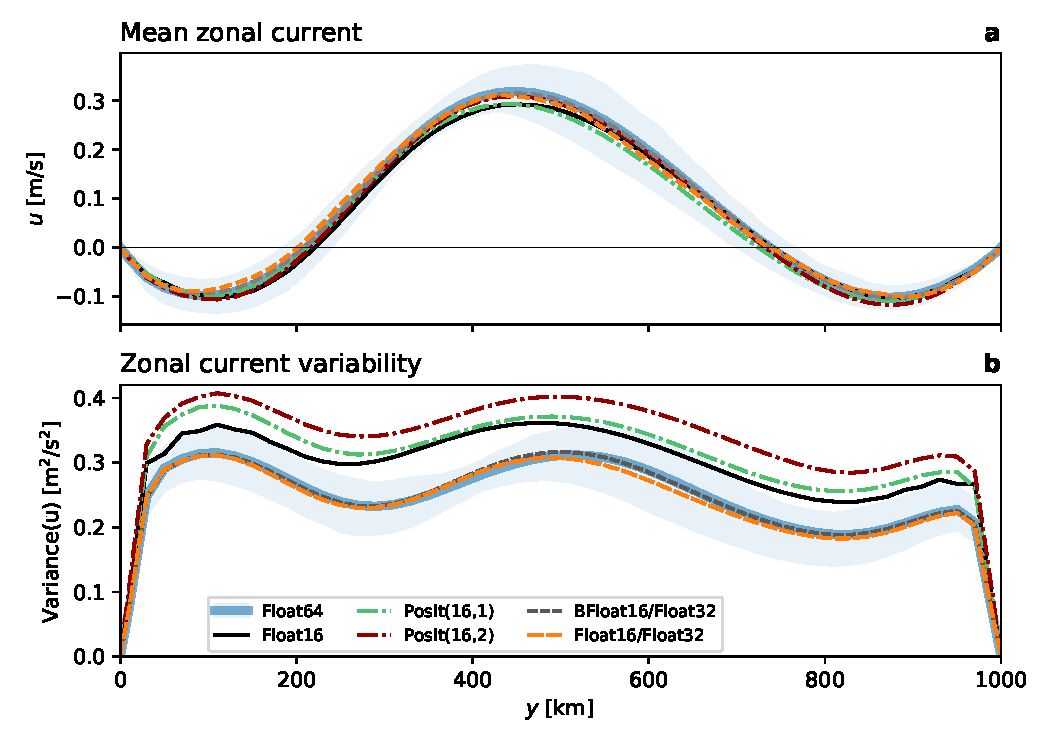
\includegraphics[width=1\textwidth]{meanvar_u.pdf}
\caption{Climatology and variability of the zonal current in the medium-resolution simulations. (a) Zonally-averaged zonal current $u$ as a function of the meridional coordinate $y$. (b) Zonal variance of the zonal current as a function of $y$. The shaded area denotes the interquartile temporal variability around the (a) mean and (b) variance of reference simulation with Float64.}
\label{fig:mean}
\end{figure}

To investigate the effect of rounding errors on the climatological mean state of the shallow water system, we zonally average the zonal velocity $u$. The mean state is an eastward flow of about 0.3~m/s, about 3 to 4 times weaker than individual velocities throughout the domain (Fig. \ref{fig:mean}a), which is typical for turbulent flows. A weak westward mean flow is found at the northern and southern boundary. No 16-bit format was found to have a significant impact on the mean state. The variability of the flow around its mean state is high throughout the domain (Fig. \ref{fig:mean}b). The variability is significantly increased by 10 -- 30\% with 16-bit arithmetic, especially with Posit(16,2). This is probably caused by rounding errors that are triggering local perturbation which increase variability.

\begin{figure}
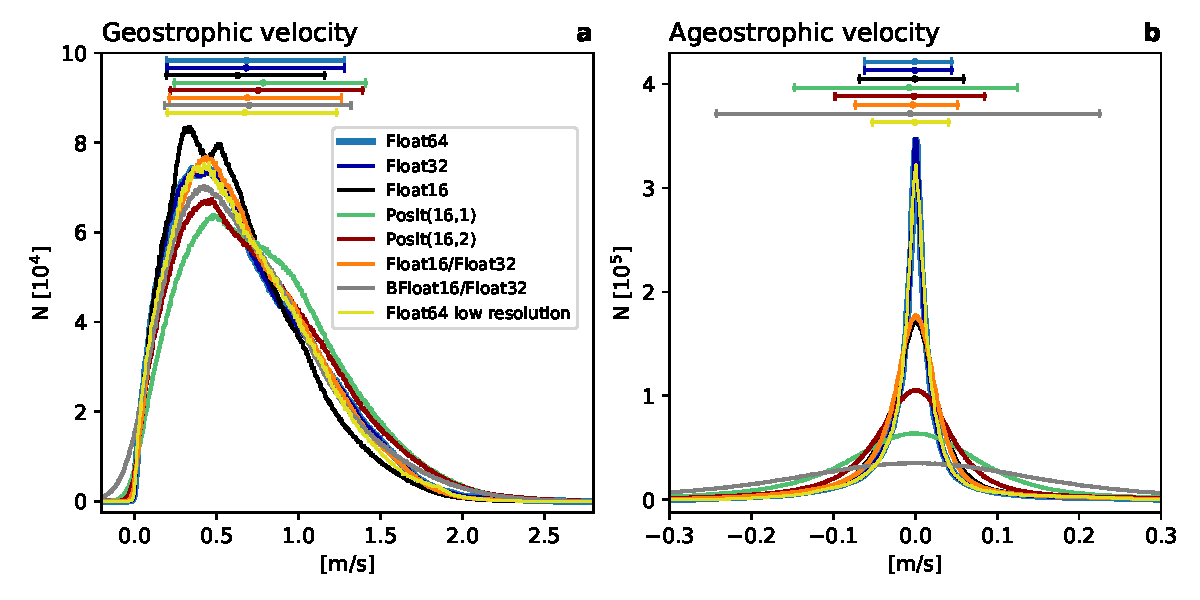
\includegraphics[width=1\textwidth]{ageostrophic.pdf}
\caption{Geostrophic balance as simulated with different number formats. (a) Histograms of flow-parallel components of geostrophic velocity. (b) as (a) but for the ageostrophic velocities. Horizontal bars denote the mean, 10th and 90th-percentile in respective colours.}
\label{fig:geo}
\end{figure}

The turbulence in shallow water simulations is largely geostrophic, such that the pressure gradient force opposes the Coriolis force. The resulting geostrophic velocities $\mathbf{u}_g$ can be derived from the sea surface height $\eta$
\begin{subequations}
\begin{align}
\mathbf{u}_g &= \frac{g}{f}\hat{\mathbf{z}} \times \nabla \eta \\
\mathbf{u} &= \mathbf{u}_{g} + \mathbf{u}_{ag}
\end{align}
\label{eq:geo}%
\end{subequations}
and deviations from the actual flow $\mathbf{u}$ are the ageostrophic velocity components $\mathbf{u}_{ag}$. We project both components on the actual velocities to obtain the flow-parallel components $\tilde{u}_{g}$ and $\tilde{u}_{ag}$ via
\begin{equation}
\tilde{u}_g = \frac{\mathbf{u}_g \cdot \mathbf{u}}{\| \mathbf{u} \|}, \quad \tilde{u}_{ag} = \frac{\mathbf{u}_{ag} \cdot \mathbf{u}}{\| \mathbf{u} \|}.
\label{eq:parallel}%
\end{equation}
The geostrophic velocities in the shallow water simulations can reach up to 2 m/s, are hardly negative (i.e. against the flow) and have a mean of about 0.7 m/s (Fig. \ref{fig:geo}a). This behaviour is well simulated with 16-bit number formats, although posits increase the strength of geostrophic velocities slightly. Ageostrophic velocity components are found to be isotropic, and are oriented equally frequent with and against the prevailing flow, but rarely exceed $\pm$0.1m/s and are therefore comparably small as expected in geostrophically balanced turbulence. Ageostrophic velocities can be seen as a measure of the physical instabilities in the flow field and their variance is indeed increased when simulated with 16-bit number formats. Float16 shows clearly fewer ageostrophic velocities around 0, pointing towards an increased number of simulated instabilities. Posits have an even further increased number of ageostrophic velocities, and especially Posit(16,1) increases the variance of those by more than factor of two. It is unclear where in the model integration rounding errors of 16-bit arithmetic trigger instabilities that lead to the observed increase in ageostrophy. We conclude that although the geostrophic balance in the simulations is maintained, rounding errors lead, likely due to an increase in ageostrophy, to a higher variability in the flow field.

\begin{figure}
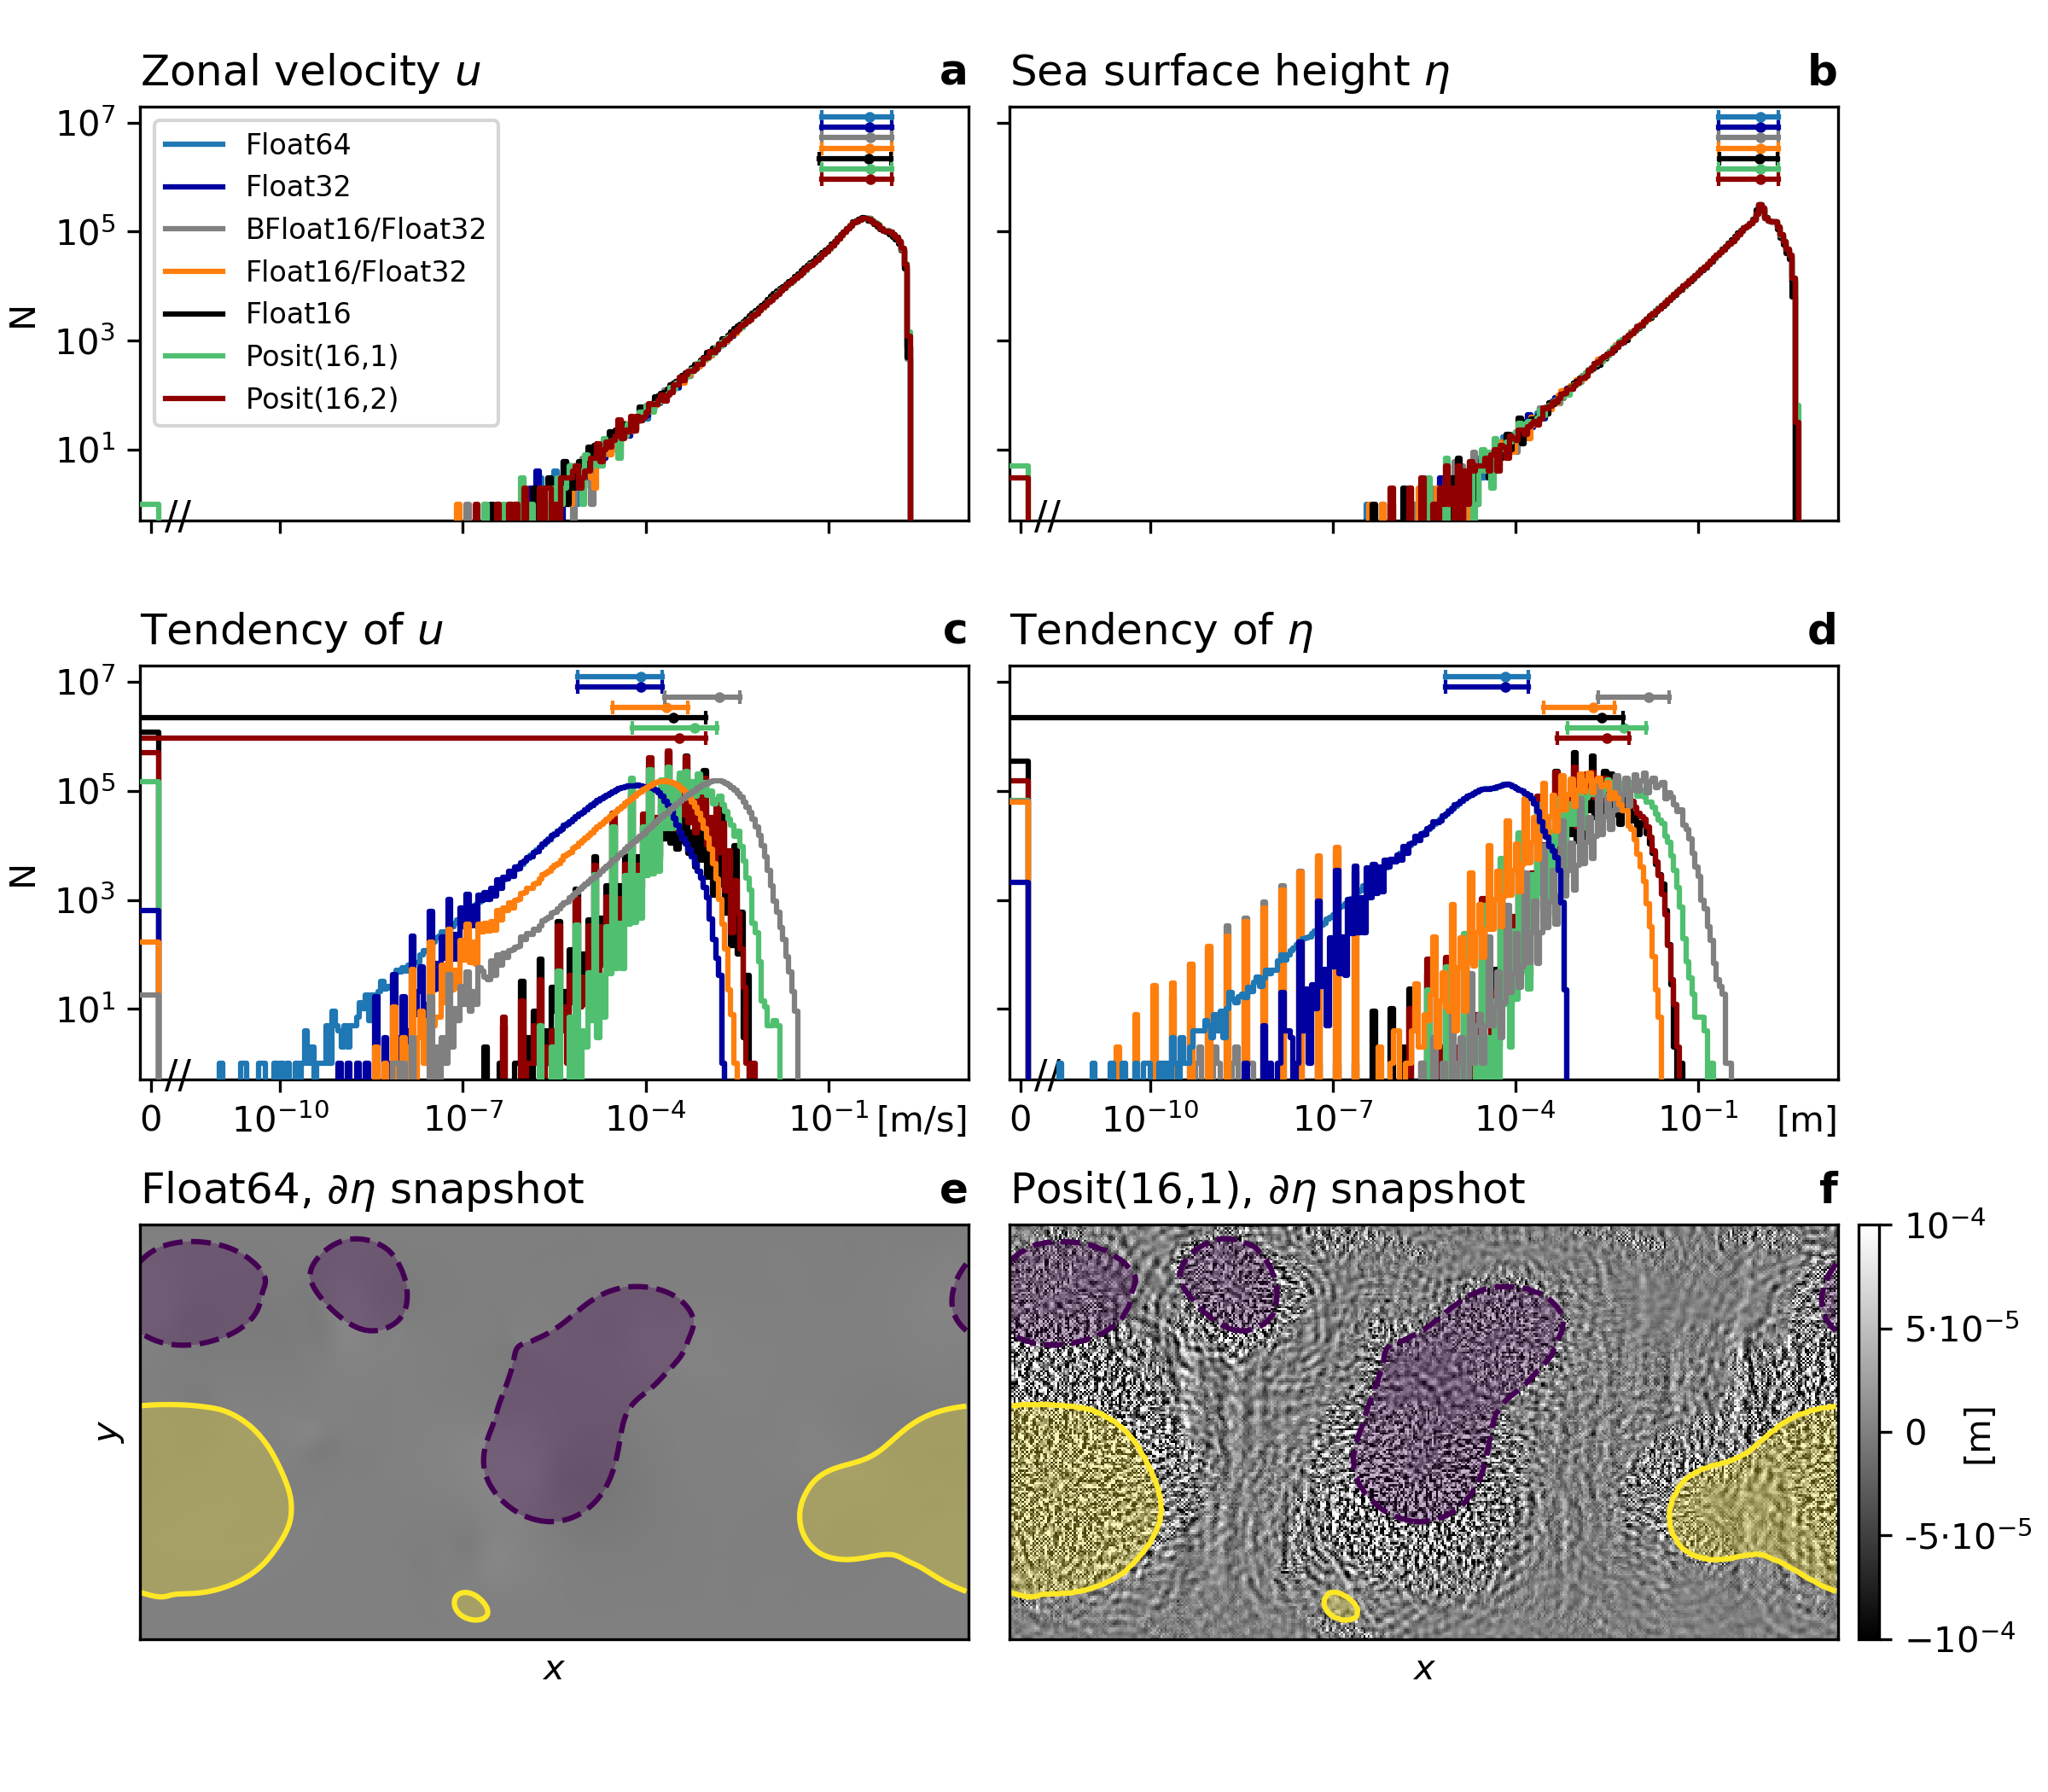
\includegraphics[width=1\textwidth]{tendency_hist.png}
\caption{Histograms of the numeric values of the prognostic variables (a) zonal velocity $u$, (b) sea surface height $\eta$, and the respective tendencies of (d) $u$ and (e) $\eta$, simulated with different 16, 32 and 64-bit number formats. Mean, 10th and 90th percentile are shown above the histograms in respective colors. Snapshots of the tendencies of $\eta$ simulated with (c) Float64 and (f) Posit(16,1). Results are similar for other 16-bit formats (not shown here). Areas of sea surface height anomalies exceeding $\pm1.4$~m are shown in purple (negativ) and yellow (positive). Note the break on the x-axis close to zero in (a,b,d) and (e).}
\label{fig:tend}
\end{figure}

As 16-bit arithmetics have no significant impact on the climatological mean state, histograms of prognostic variables are also not changed (Fig. \ref{fig:tend}a and b). However, the tendencies are increased by orders of magnitude with 16-bit arithmetics (Fig. \ref{fig:tend}d and e), as rounding errors cause gravity waves to radiate away from eddies (Fig. \ref{fig:tend}f). Gravity waves are identified from the tendency of sea surface height. Comparing their propagation to the location of anomalous sea surface height, which is used as a proxy for eddies, we assume that rounding errors in regions of high eddy activity lead to instabilities that propagate away in the form of gravity waves. These gravity waves are not present in Float64 simulations (Fig. \ref{fig:tend}c) and tend to have only a small impact on quasi-gestrophic dynamics, as they act on different time and length scales. It is unclear whether these gravity waves cause the observed ageostrophic velocities.

The tendencies are about 4 orders of magnitude smaller than the prognostic variables. This poses a problem for number formats with a machine epsilon, measured as decimal precision, significantly lower than 4 decimal places (Table \ref{tab:formats}). Float16 has a machine epsilon of 3.7, which is presumably close to the lower limit beyond which the addition of tendencies will be round back. The BFloat16 number format has a machine error of 2.8, which explains why no change from initial conditions in the shallow water system can be simulated with BFloat16.

\subsubsection{Mixed precision arithmetic in the shallow water model}
\label{sec:mixed}

In the previous simulations the entire shallow water simulation was performed with the specified number format. As the addition of tendencies to the prognostic variables was identified as a key calculation that is error-prone, we investigate now the benefits of mixed precision arithmetic, where Float32 is used for the prognostic variables but the tendencies are computed with either Float16 or BFloat16, two number formats that have the lowest decimal precision for numbers around 1. The prognostic variables are now reduced to Float16 or BFloat16 before calculations of the right-hand side and every term of the tendencies is converted back before addition to the prognostic variables. Using subscripts 16 and 32 to denote variables held at 16 and 32-bit precision, respectively, and let Float32() be the conversion function then the continuity Eq. \ref{eq:swe}b becomes
\begin{equation}
\frac{\partial \eta_{32}}{\partial t} = -\op{Float32}( \partial_x(u_{16}h_{16}) + \partial_y(v_{16}h_{16} ))
\label{eq:conversion}
\end{equation}
and similar for $u$ and $v$ in Eq. \ref{eq:swe}a.

Snapshots of tracer concentration reveal well simulated geostrophic turbulence (Fig. \ref{fig:snapshot}e and f) with Float16/Float32 or BFloat16/Float32 and instabilites at fronts or in filaments are visibly reduced compared to pure 16-bit arithmetic. The forecast error is strongly reduced once the prognostic variables are kept as Float32 (Fig. \ref{fig:rmse}a), supporting the hypothesis that the addition of tendencies to the prognostic variables is a key computation with low rounding error-tolerance. Despite BFloat16 not being suitable for shallow water simulations when applied to all computations, mixing BFloat16 with Float32 arithmetic yields a similar error growth to posits, which is well below the discretization error. Mean state or variability are virtually identical for both mixed precision cases (Fig. \ref{fig:mean}) compared to the Float64 reference. The geostrophic balance is largely unaffected, but ageostrophic velocities increase in variance, especially for BFloat16 (Fig. \ref{fig:geo}). Gravity waves are similarly present for mixed precision although weaker for tendencies computed with Float16 (Fig. \ref{fig:tend}d) and, as discussed, they tend to not interact with the geostrophic time and length scales. Although the results show that Float16 is generally a preferrable number format over BFloat16 for the applications presented here, we acknowledge that the conversion between Float32 and Float16 will come with some computational cost. In contrast, the conversion between BFloat16 and Float32 is computationally very cheap as both formats have the same number of exponent bits. Removing signifcant bits, potentially applying rounding, and padding trailing zeros, are the only operations for this conversion. Following the results here, mixing 16 and 32 bit precision is found to be a possible solution to circumvent spurious behaviour due to 16-bit floating-point arithmetics. Performance benefits are still possible as most calculations are performed with 16 bit, with key computations in 32 bit to reduce the overall error. Depending on the application, the conversions between number formats are assumed to be of negligible cost. This is an attractive solution as hardware-accelerated 16-bit floating-point arithmetic is already available on graphic or tensor processing units and implementations therefore do not rely on the development of future computing hardware, as it is the case for posits.

\begin{figure}
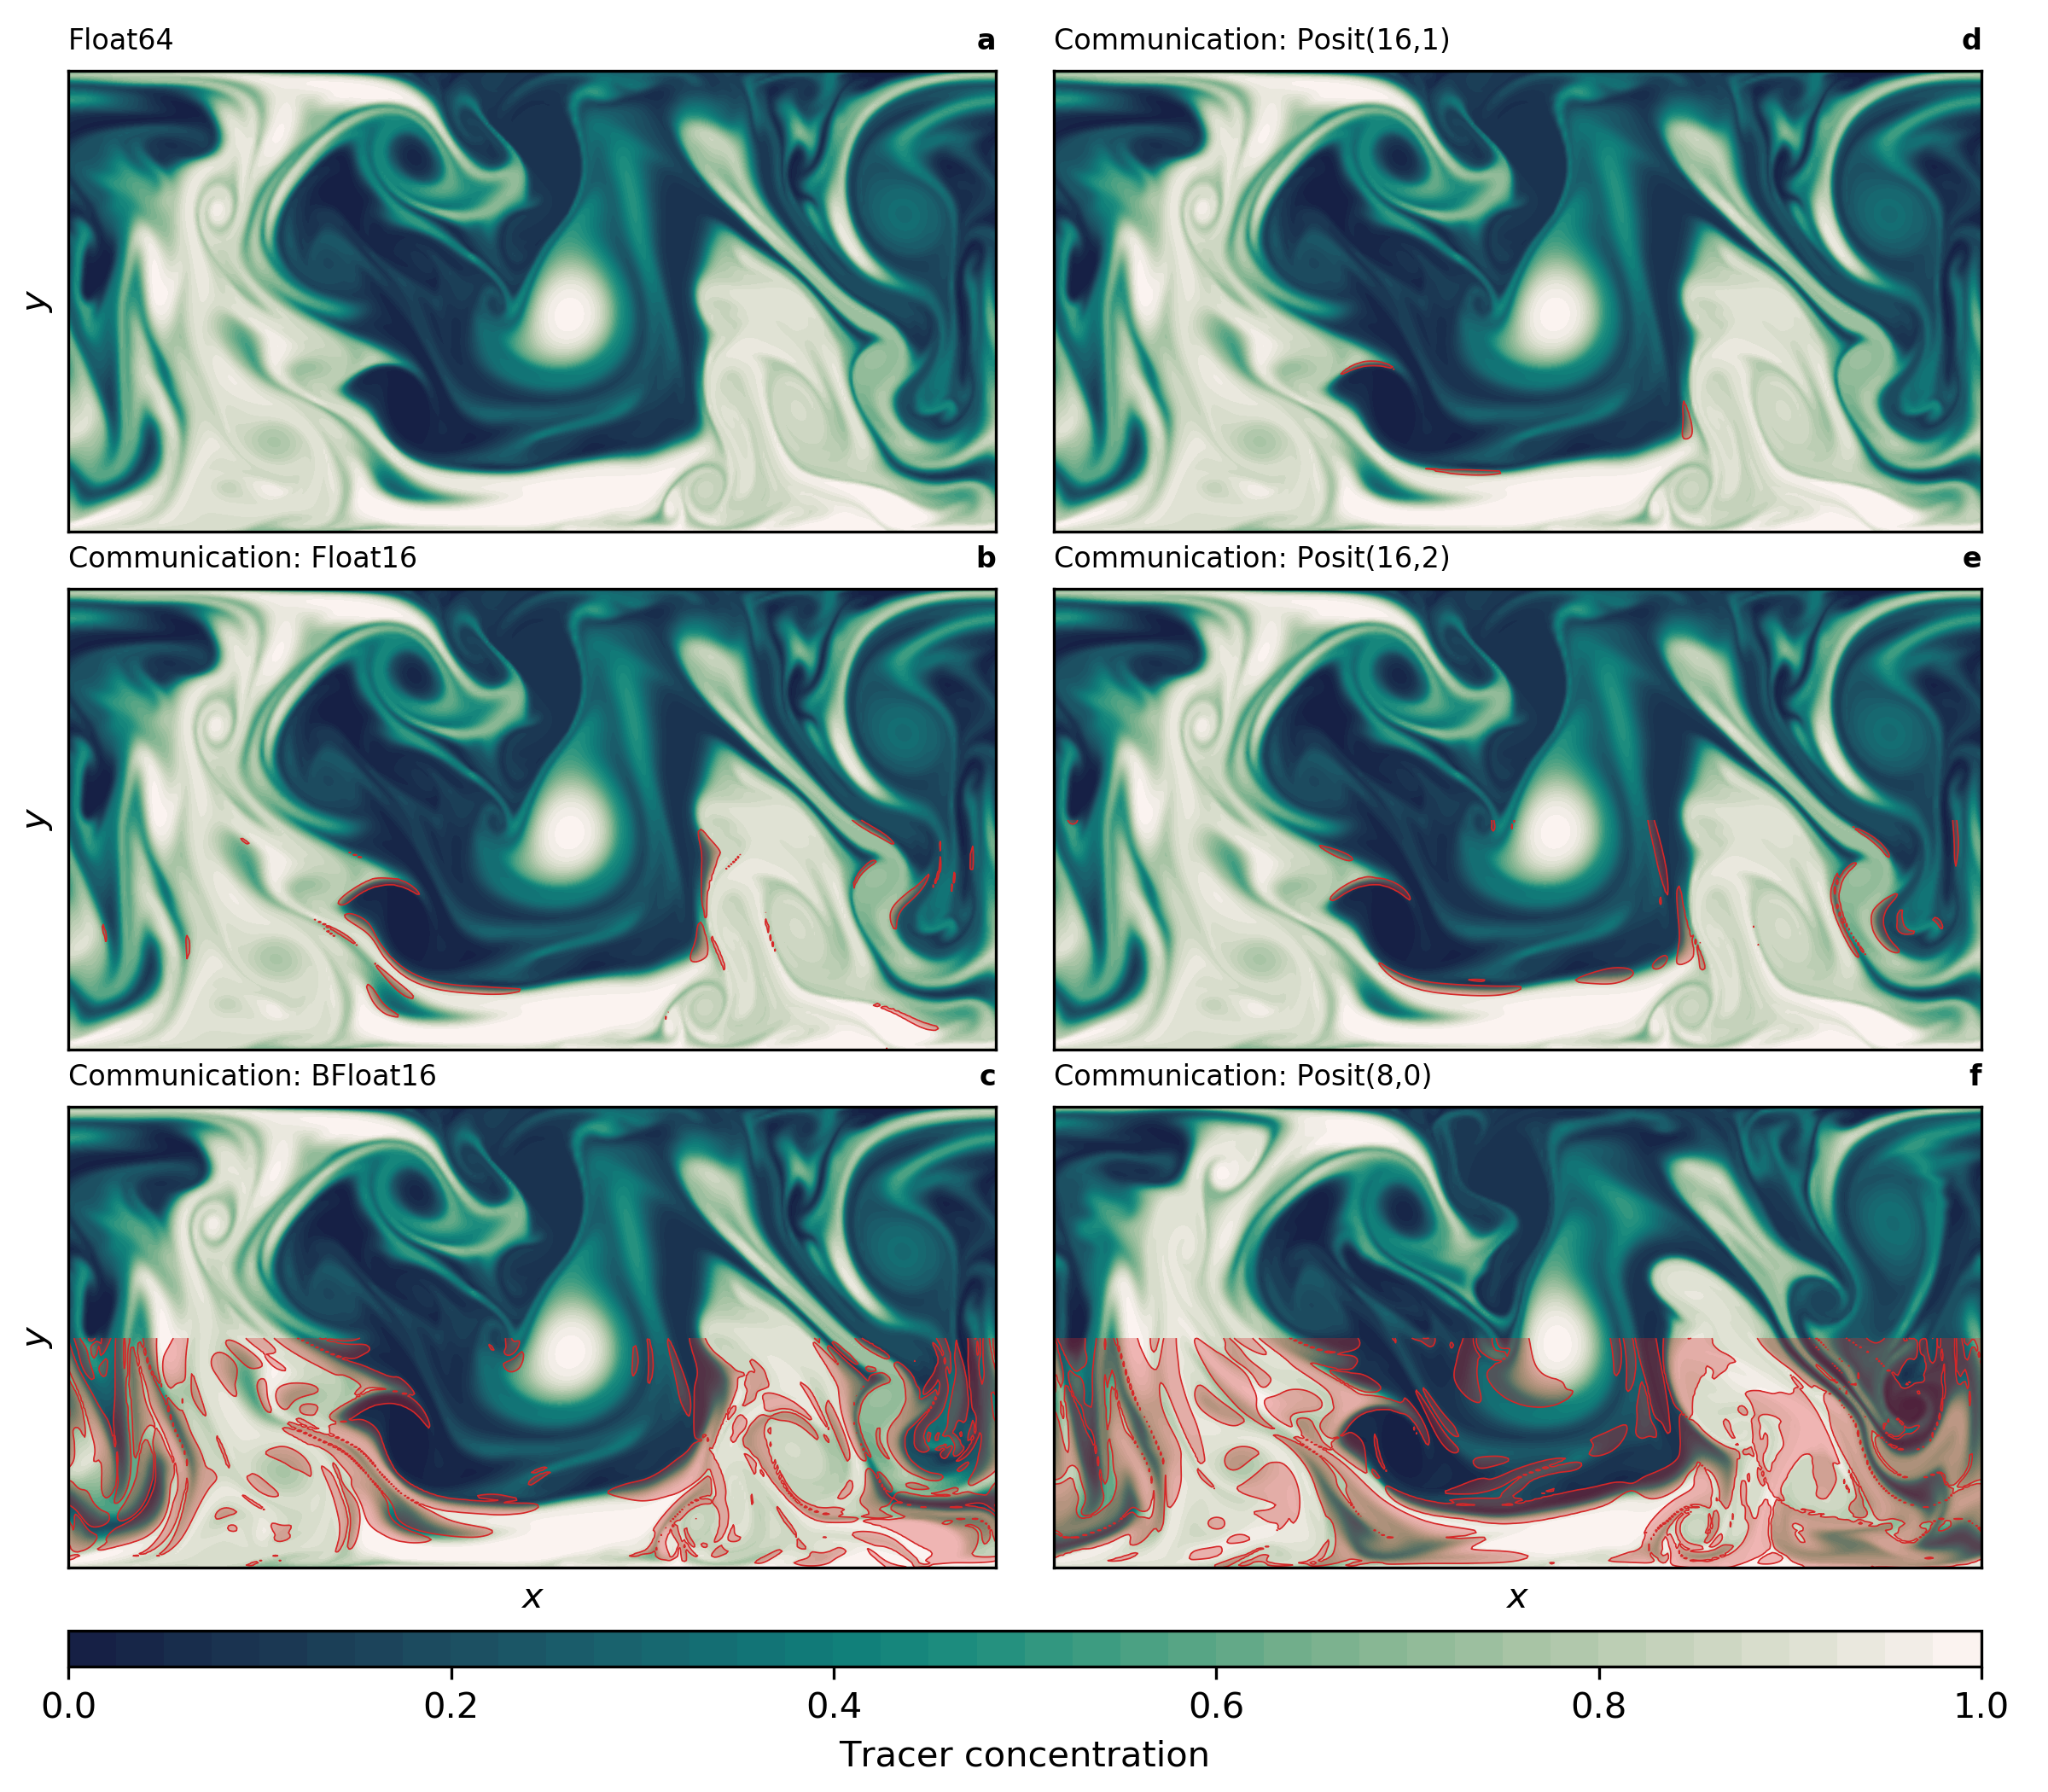
\includegraphics[width=1\textwidth]{snapshot_comm.png}
\caption{Snapshot of tracer concentration simulated by the shallow water model using reduced precision communication. The communication of boundary values occurs at every time step for the prognostic variables. Float64 was used for all calculations. Areas where the absolute error exceeds 0.05 are shaded in red only in the lower half of the domain. The tracer was injected uniformly in the lower half of the domain 50 days before. This simulation was run with the high-resolution configuration.}
\label{fig:snapshot_comm}
\end{figure}


\subsubsection{Reduced precision communication for the shallow water model}
\label{sec:comm}

A standard method to parallelise simulations is the distributed-memory parallelism via Message Passing Interface (MPI). We emulate MPI-like communication in the shallow water model with the copying of boundary values between the right and left boundary (periodic boundary conditions). Although the shallow water model does not run in parallel, reducing the precision in the copying of boundary values introduces an equivalent error as if reduced precision MPI was used to communicate between subdomains. Reduced precision is applied for the communication of the prognostic variables at every Runge-Kutta substep.

Regarding snapshots of tracer concentration simulated with reduced precision communication show a negligible error for Float16 and posits (Fig. \ref{fig:snapshot_comm}). The error is largest at fronts and not concentrated around the boundaries. Encoding the communication with BFloat16 introduces a larger error than for the other 16-bit formats as the decimal precision is with 2.8 clearly lower (Table \ref{tab:formats}) for the range of values occuring within the prognostic variables (Fig. \ref{fig:tend}a and b). The errors are quantified by the RMSE of surface height $\eta$ as before and are up to about two orders of magnitude smaller than the errors that result from 16-bit arithmetic. As even the worst 16-bit communication format, BFloat16, has a smaller error than the best mixed precision formats, Float16 with Float32, we extend the short-term forecast experiments to include two 8-bit formats, Posit(8,0) and Float8 (see Table \ref{tab:formats} for a description). Both formats are found to be suitable for reduced precision communication here and do not introduce an error that is larger than the discretization error. Having said that, Float8 communication introduces an error that is comparably large initially but growths only linearly in the first 50 days of the simulation, which is in contrast to the exponential error growth observed for 16-bit arithmetic.


\section{Conclusion and Discussion}
\label{sec:discuss}

Running computationally demanding algorithms at 16-bit could reduce the wall-clock time for weather and climate simulations on future high performance computing architecture.
Using a software emulator, we have tested a number of options for 16-bit arithmetic for weather and climate applications.
We achieved the best results with 16-bit posits (with either 1 or 2 exponent bits) which appear very promising for application in high performance computing for Earth System modelling.
Float16 can be used to perform forecasts with the shallow water model while the application of BFloat16 or integer arithmetic was not successful.
In general, 16-bit arithmetics were not found to alter the climatological mean state or the large-scale dynamics.
However, variability and ageostrophic velocities were increased, such that second and higher-order statistics should undergo testing to assess the models reliability.
Depending on the application, an increased variability does not necessarily deteriorate the model, especially for more realistic model set-ups as considered here.

In general, 16-bit arithmetics were not found to alter the mean fields or the large-scale dynamics.
However, variability and ageostrophic velocities were increased. Depending on the application, an increased variability does not necessarily deteriorate the model, especially for more realistic model configurations that take model error into account, for example by using stochastic parametrisation schemes. However, this finding suggests that reduced precision changes need to be done carefully as specific model features can change properties without visible impact on mean diagnostics.

To enable shallow water simulations with 16-bit arithmetic required the rearrangement of a couple of terms but no major revisions of the model code or algorithms.
Given that only floats are currently hardware-supported, we investigated mixed precision approaches, where the prognostic variables are kept at 32 bit and the tendencies are computed in 16 bit and found that the impact of rounding errors can be reduced significantly.
We also showed that numerical precision for communication between compute nodes can be greatly reduced down to 16 or even 8-bit without introducing a large error.
Reduced precision communication was not found to have a significant impact on either mean state, variability, geostrophy or tendencies.

In this study, we perform model forecasts with a \emph{perfect model}.
Any form of model error is ignored, as the Float64 reference is exactly the same model as its reduced precision counterparts and any form of initial condition error is also ignored.
Only discretisation errors are estimated by lowering the spatial resolution by a factor of 2.
This is not a realistic set-up for weather or climate models.
Real models include many other sources of forecast error and it is likely that the contributions of rounding errors from 16-bit arithmetic would be dwarfed by errors in initial conditions or discretisation errors in many applications.

The numerical discretisation that was used for the shallow water model in this paper, with an explicit time stepping scheme and 2nd order centred finite differences, is common to solve the equations of motion in fluid dynamics.
However, various different methods of discretisation exist, including spectral methods, finite element/volume and implicit time stepping.
The requirements on reduced precision will differ for the different algorithms and some methods may be more sensitive to rounding errors compared to the techniques that were studied here.

As there is no hardware available for posit arithmetic that we could have used for performance testing, we cannot draw any conclusion about the performance of posit arithmetic operations in comparison to Float16 or the other formats.
Until progress is made on hardware implementations for posits, the results here suggest that also 16-bit float arithmetic can succesfully be used for parts of complex weather and climate models with the potential for acceleration on graphic and tensor processing units.
It is therefore recommended to adapt a type-flexible programming paradigm, ideally in a language that supports portability, with algorithms written to reduce the dynamic range of arithmetic results.
Hardware progress on central, graphic or tensor processing units, with various numbers formats supported, can subsequently be utilised to accelerate weather and climate simulations.


\acknowledgments
Milan Kl\"{o}wer and Tim N. Palmer gratefully acknowledge funding by the European Research Council under grant number 741112 \emph{An Information Theoretic Approach to Improving the Reliability of Weather and Climate Simulations}. Milan Kl\"{o}wer is also funded by NERC grant number NE/L002612/1.  Peter D. D\"{u}ben gratefully acknowledges funding from the Royal Society for his University Research Fellowship as well as funding from the ESIWACE2 project. ESIWACE2 has received funding from the European Union's Horizon 2020 research and innovation program under grant agreement 823988.

Data and scripts will be available at
\url{https://github.com/milankl/ClimateModels16bit} upon acceptance. Relevant software is available via \url{https://github.com/milankl} in the following repositories: SoftPosit.jl, ShallowWaters.jl, Lorenz63.jl, and Float8s.jl.

\bibliography{bibliography}

\end{document}
